% -*- mode: latex; coding: utf-8 -*-
% !TEX TS-program = pdflatexmk
% !TEX encoding = UTF-8 Unicode

\RequirePackage[hyphens]{url}
\documentclass[%
  a4paper,
  twoside,
  numbers=noenddot,
  parskip=half,
  open=any,
  headsepline,
  english, % german, english
  ba  % ba, pa
]{zhawthesis}

\usepackage{etoolbox}


%%%%%%%%%%%%%%%%%%%%%%%%%%%%%%%%%%%%%%%%
% Parameters
% - Adjust these to your needs:

\title{Functional Go}
\subtitle{...An Easier Introduction to Functional Programming}
\author{% Komma getrennt
    Ramon Rüttimann
}
\newcommand\twodigits[1]{\ifnum#1<10 0#1\else #1\fi}
\date{\twodigits{\the\day}.\twodigits{\number\month}.\the\year}

\major{Computer Science}  % Studiengang
\zhawsemester{Spring 2020}
\zhawinstitute{init}
\zhawlogocolour{pantone2945}  % pantone2945, cmyk, sw
\mainsupervisor{Dr. G. Burkert}
\subsupervisor{Dr. K. Rege}

%%%%%%%%%%%%%%%%%%%%%%%%%%%%%%%%%%%%%%%%
% Base packages used by the template (any commonly used packages)

%\PassOptionsToPackage{hyphens}{url}\usepackage{hyperref}

\usepackage{float}
\usepackage{graphicx}
\graphicspath{{figures/}}
\DeclareGraphicsExtensions{.pdf,.png,.jpg,.gif}

\usepackage{tabularx}
\usepackage{longtable}
\usepackage{booktabs}
\usepackage{todonotes}

%%%%%%%%%%%%%%%%%%%%%%%%%%%%%%%%%%%%%%%%
% Custom packages
% - Add packages used by your thesis here:

%\usepackage{hyperref}
%\PassOptionsToPackage{hyphens}{url}\usepackage{hyperref}

\usepackage[newfloat]{minted}
\usepackage{listings}
\newenvironment{code}{\captionsetup{type=listing}}{}
\SetupFloatingEnvironment{listing}{name=Source Code,placement=H}
\definecolor{bg}{rgb}{0.95,0.95,0.95}
\newminted{bash}{breaklines,breakbytoken,tabsize=2,bgcolor=bg}
\newminted{bnf}{breaklines,breakbytoken,tabsize=2,bgcolor=bg}
\newminted{c}{breaklines,breakbytoken,tabsize=2,bgcolor=bg}
\newminted{go}{breaklines,breakbytoken,tabsize=2,bgcolor=bg}
\newminted{haskell}{breaklines,breakbytoken,tabsize=2,bgcolor=bg}
\newminted{java}{breaklines,breakbytoken,tabsize=2,bgcolor=bg}
\newmintedfile{go}{breaklines,breakanywhere,tabsize=2,bgcolor=bg,linenos,stepnumber=5,numberfirstline}


\newcommand{\gofilerange}[4][]{%
    \immediate\write18{./utils/delim -file="#2" -start="#3" -end="#4"}
    \IfFileExists{code.lineno}
      {\CatchFileEdef{\linenumber}{./code.lineno}{\endlinechar=-1 }}
      {\def\linenumber{0}}
    \edef\flags{firstnumber=\linenumber,#1}
    \expandafter\gofile\expandafter[\flags]{./code.snippet}
}

%\sloppy

\usepackage[
    backend=biber,
    style=ieee,
    dashed=false,
]{biblatex}
\usepackage{xurl}
\usepackage{caption}
\usepackage[toc,page]{appendix}
\usepackage{glossaries}
%\usepackage{listings}
\makeglossaries
%\usepackage{csquotes}
\AtBeginEnvironment{quote}{\itshape}
%\bibliography{thesis}
\addbibresource{thesis.bib}

\begin{document}

\frontmatter

\maketitle

\cleardoublepage % chktex 1


%%%%%%%%%%%%%%%%%%%%%%%%%%%%%%%%%%%%%%%%
% Declaration of Originality

\makedeclarationoforiginality % chktex 1


\cleardoublepage % chktex 1


%%%%%%%%%%%%%%%%%%%%%%%%%%%%%%%%%%%%%%%%

\IfLanguageName{nswissgerman}{\chapter{Zusammenfassung}}{\chapter{Summary}}
\label{ch:summary} % chktex 24
% -*- mode: latex; coding: utf-8; TeX-master: ../thesis -*-
% !TEX TS-program = pdflatexmk
% !TEX encoding = UTF-8 Unicode
% !TEX root = ../thesis.tex

Innerhalb der letzten zehn Jahre haben Konzepte und Ideen aus dem funktionalen
Programmieren im Alltag von vielen Entwicklern Fuss gefasst. Häufig wird
empfohlen, eine pur funktionale Programmiersprache wie zum Beispiel Haskell
zu lernen, um sich mit diesen Konzepten vertraut zu machen. Viele haben jedoch
Mühe, eine neue Syntax und ein neues Paradigma gleichzeitig zu lernen. Das Ziel
dieser Arbeit ist deswegen, einen einfacheren Einstieg in funktionales Programmieren
zu ermöglichen, dies mit Hilfe einer multiparadigmatischen Programmiersprache mit bekannter
Syntax.

Um dieses Ziel zu erreichen, wurde die Programmiersprache Go aufgrund ihrer
syntaktischen Simplizität und Vertrautheit gewählt.
Da Listen jedoch oft eine zentrale Rolle im funktionalen Programmieren einnehmen, ist ein
Nachteil dieser Wahl, dass Go keinen eingebauten List Datentyp besitzt. Zwar wird
dieser Nachteil durch Go's `Slices' gemildert, jedoch fehlen viele sogenannte `higher-order'
Funktionen um mit Listen zu arbeiten --- `map', `filter' und `reduce', um einige zu nennen.
Da Go's Typensystem keinen Polymorphismus bietet, müssen diese Funktionen im Compiler
implementiert werden, um eine möglichst benutzerfreundliche Verwendung zu ermöglichen.

Zusätzlich dazu wird die Bedeutung von `pure functional Programming' im Kontext dieser Arbeit
festgelegt und auf Basis dieser Definition das Code-Analyse Tool `funcheck' entwickelt, welches
nicht-funktionale Konstrukte im Programmcode meldet.

Mit den neuen built-in Funktionen `fmap', `filter', `foldr', `foldl' und `prepend',
sowie dem Linter `funcheck' erweist sich Go als geeignete Programmiersprache um
einen einfachen Einstieg in funktionales Programmieren zu ermöglichen. Der primäre Grund
spiegelt sich auch im Go Idiom `clear is better than clever' wider. Obwohl funktionaler
Go Code länger ist als in funktionalen Sprachen, ist dieser auch einfacher nachzuvollziehen.
Des Weiteren zeigt die Arbeit aber auch, dass es keinen Weg um eine pure funktionale Sprache
wie Haskell gibt, um sich funktionales Programmieren vollständig anzueignen.
Haskell's zwar ungewöhnliche, aber prägnante Syntax sowie das Design
der Sprache --- das Typensystem, Pattern Matching, die Purity Guarantees und vieles mehr ---
bilden hierfür eine solide und oft verwendete Grundlage.


\chapter{Abstract}
\label{ch:abstract} % chktex 24
% -*- mode: latex; coding: utf-8; TeX-master: ../thesis -*-
% !TEX TS-program = pdflatexmk
% !TEX encoding = UTF-8 Unicode
% !TEX root = ../thesis.tex

In the last decade, concepts from functional programming have grown in
importance within the wider, non-functional programming community.
Often it is recommended to learn a purely functional programming language
like Haskell to become familiar with these concepts.
However, many programmers struggle with the double duty
of learning a new paradigm and a new syntax at the same time. Because of
this, this paper expands on the idea of learning purely functional programming
with a multi-paradigm programming language with a familiar syntax. The Go
programming language has been the choice for this due to its syntactical
simplicity and familiarity.

The absence of a list datatype in Go is remediated by Go's slices.
However, Go is missing the typical higher-order functions ---
`map', `filter' and `fold' to name a few --- that are present in every
functional programming language and many other programming languages too. Due to
this, the most popular higher-order functions have been determined and, because of the
absence of polymorphism in Go, implemented as built-in functions in the compiler.

Furthermore, this paper specifies a definition of what pure functional programming is and
introduces `funcheck', a static code analysis tool that has been designed and implemented to
report constructs that are non-functional.

With the help of the newly built-in functions `fmap', `filter', `foldr', `foldl' and
`prepend', as well as `funcheck' to lint code, Go proves itself to be a
suitable language for getting started with functional programming.
At the same time, it also shows that there is no way around learning a
language like Haskell if fluency with functional programming concepts
is desired. The primary reasons are that, although it may be unusual, Haskell's
syntax is extremely concise, and that the language's design --- the type system,
pattern matching, the purity guarantees and more --- provides a very effective toolset
for purely functional programming.


\IfLanguageName{nswissgerman}{\chapter{Vorwort}}{\chapter{Preface}}
\label{ch:preface} % chktex 24
% -*- mode: latex; coding: utf-8; TeX-master: ../thesis -*-
% !TEX TS-program = pdflatexmk
% !TEX encoding = UTF-8 Unicode
% !TEX root = ../thesis.tex

As a part of my bachelor studies, I chose to attend a course on functional programming.
Having worked with Go for the last 3 years, first-class and higher-order functions
were not particularly new ideas to me. However, learning Haskell was, at the beginning,
overwhelming.

So I rewrote some exercises that I did not understand in Go.
%So what I did for some exercises that I could not understand completely is that
%I rewrote them in Go.
The result was more verbose; usually
roughly two to three times the lines of code for the same algorithm.
However, after writing the Go version, I understood not only the Go version,
but also the Haskell version.

After doing this a couple of times, I realised that I was constantly rewriting
the same higher-order functions with different types, but more or less the same
implementation. Thus, the idea of adding them as built-ins came up.

`Funcheck' then came into play when I wanted to build something in Go first and
then rewrite it in Haskell. It was hard to tell whether it was purely functional,
but it needed to be in order to be easier to write the implementation in Haskell.

This thesis is written based on my own struggles I had with Haskell, and it is
my hope that someday, someone may benefit from the work done in this thesis.

Special thanks to:

My supervisors Gerrit Burkert and Karl Rege for their support and guidance,
Tom Whiston for proofreading this thesis and improving my English,
Eva Kuske for the consultation on writing and
my employer nine (\href{http://nine.ch}{nine.ch}) for their flexible working times.


\cleardoublepage % chktex 1


%%%%%%%%%%%%%%%%%%%%%%%%%%%%%%%%%%%%%%%%
\mainmatter % chktex 1

\tableofcontents

\IfLanguageName{nswissgerman}{\chapter{Einleitung}}{\chapter{Introduction}}
\label{ch:introduction} % chktex 24
% -*- mode: latex; coding: utf-8; TeX-master: ../thesis -*-
% !TEX TS-program = pdflatexmk
% !TEX encoding = UTF-8 Unicode
% !TEX root = ../thesis.tex

\section{Learning Functional Programming}
\todo[inline]{
    rewrite first sentence. Also, Rust being 'more popular' is dangerous, too.
    Less vague expressions, "seems to be", "and many more".
    Java 8 added a lot of functional features, C\# too.
}
When Javascript and Python started to take off around 2010\autocite{python-popularity},
they also brought rise to a lot of concepts borrowed from functional programming.
Since then, many new multi-paradigm
languages have appeared and gotten more popular, as for example Go, Rust,
Kotlin and Dart.
Most of the languages mentioned support an imperative, object-oriented, as well as a functional programming style.
Rust, being the `most popular programming language'%\autocite{rust-loved}%
for 4 years in a row (2016--2019), has been
significantly influenced by functional programming languages\autocite{rust-functional} and borrows a lot of functional
concepts in idiomatic Rust code.

Learning a functional programming language increases fluency with these concepts and teaches a different
way to think and approach problems when programming. For those reasons, and many more, a lot of programmers
advocate learning a functional programming language.

Though the exact definition of what a \textit{purely} functional language consists of remains a controversy\autocite{functional-controversy},
the most popular, pure functional programming language seems to be Haskell\autocite{comparison-functional-languages}.

\section{Haskell}

Haskell, the \textit{lingua franca} amongst functional programmers, is a lazely-evaluated, purely functional programming
language. While Haskell's strengths stem from all it's features like type classes, type polymorphism, purity and more,
these features are also what makes Haskell famously hard to learn\autocite{haskell-hard-one}\autocite{haskell-hard-two}\autocite{haskell-hard-three}\autocite{haskell-hard-four}.

Beginner Haskell programmers face a very distinctive challenge in contrast to learning a new, non-functional programming language:
Not only do they need to learn a new language with an unusual syntax (compared to imperative or object-oriented languages), they
also need to change their way of thinking and reasoning about problems.
For example, the renowned quicksort-implementation from the Haskell Introduction Page\autocite{haskell-quicksort}:

\begin{haskellcode}
quicksort :: Ord a => [a] -> [a]
quicksort []     = []
quicksort (p:xs) = (quicksort lesser) ++ [p] ++ (quicksort greater)
    where
        lesser  = filter (< p) xs
        greater = filter (>= p) xs
\end{haskellcode}

While this is only a very short and clean piece of code, these 6 lines already pose many challenges to non-experienced Haskellers;

\begin{itemize}
    \item The function's signature with no `fn' or `func' statement as they often appear in imperative languages
    \item The pattern matching, which would be a `switch' statement or a chain of `if / else' conditions
    \item The deconstruction of the list within the pattern matching
    \item The functional nature of the program, passing `(< p)' (a function returning a function) to another function
    \item The function call to `filter' without paranthesised arguments and no clear indicator at which arguments
        it takes and which types are returned
\end{itemize}

Though some of these points are also available to programmers in imperative or object-oriented languages, the cumulative difference
is not to underestimate and adds to Haskell's steep learning curve.

 %TODO: talk about production-ready code and programmers?

\section{Goals}

\todo[inline]{unclear first sentence, not specific enough}

The goal is to solve the issue of the first steps in functional programming.
Learning a new paradigm and syntax at the same time can be daunting and discouraging for novices.
By using a modern, multi-paradigm language with a clear
and familiar syntax, the functional programming beginner should be able to focus on the paradigm
first, and then change to a language like Haskell to fully get into functional programming.

To ease the learning curve of functional programming, this thesis will consist of two parts:

\todo[inline]{should not be a list, for the flow}
\begin{itemize}
    \item Make a multi-paradigm language support functional programming as much as needed.
        The criteria for this language are:
    \begin{itemize}
        \item Easy, familiar syntax
        \item Be statically typed, as this makes it easier to reason about a program
        \item Have support for functional programming features like first class functions, currying
            and partial application
    \end{itemize}
    \item Create a linter that checks code on its functional purity. For this, some rules will have
        to be curated to define what pure functional code is.
\end{itemize}

It s not the goal to create a production-ready functional language, so runtime and performance requirements
can be ignored.

\section{Why Go}

The language of choice for this task is Go, a statically typed, garbage-collected programming language
designed at Google in 2009\autocite{golang-publish}. With its strong syntactic similarity to C, it should
be familiar to most programmers.
Go is an extremely verbose language with almost no syntactic sugar. This makes it a perfect fit to
grasp the concepts and trace the inner workings of functional programming.

There are, however, a few downsides of using Go:

% TODO: should not be a list.
\todo[inline]{shouldn't be a list either}
\begin{itemize}
    \item No polymorphism. Go 2 will likely have support for polymorphism, but at the time of writing,
        there is no implementation available.
    \item Missing implementations for common functions like `map', `filter', `reduce' and more.
    \item No list implementation. Go has `slices', which are `views' on arrays, but
        no list datatype.
\end{itemize}

\subsection{Go Slices}

Go's Slices can be viewed as an abstraction over arrays, to mitigate some of the weaknesses of arrays
compared to lists.

\begin{quote}
    Arrays have their place, but they're a bit inflexible, so you don't see them too often in Go code.
    Slices, though, are everywhere. They build on arrays to provide great power and convenience.\autocite{golang-slices}
\end{quote}

Slices can be visualised as a `struct' over an array:

\begin{gocode}
// NOTE: this type does not really exist, it
// is just to visualise how they are implemented.
type Slice struct {
    // the underlying "backing store" array
    array *[]T
    // the length of the slice / view on the
    //array
    len   int
    // the capacity of the array from the
    // starting index of the slice
    cap   int
}
\end{gocode}

With the `append' function, elements can be added to a slice. Should the underlying array not have enough
capacity left to store the new elements, a new array will be created and the data from the old array will
be copied into the new one. This happens transparently to the user.

\subsubsection{Using Slices}

`head', `tail' and `last' operations can be done with index expressions:

\begin{gocode}
// []<T> initialises a slice, while [n]<T> initialises an
// array, which is of fixed length n. One can also use `...'
// instead of a natural number, to let the compiler count
// the number of elements.
s := []string{"first", "second", "third"}
head := s[0]
tail := s[1:]
last := s[len(s)-1]
\end{gocode}

Adding elements or joining slices is achieved with `append':

\begin{gocode}
s := []string{"first", "second"}
s = append(s, "third", "fourth")
t := []string{"fifth", "seventh"}
s = append(s, t...)
// to prepend an element, one has to create a
// slice out of that element
s = append([]string{"zeroth"}, s...)
\end{gocode}

Append is a variadic function, meaning it takes \textit{n} elements. If the slice is of type \textit{[]<T>},
the appended elements have to be of type \textit{<T>}.

To join two lists, the second list is expanded into
variadic arguments.

More complex operations like removing elements, inserting elements in the middle or finding
elements in a slice require helper functions, which have also been documented in Go's
Slice Tricks\autocite{slice-tricks}.

\subsubsection{What is missing from Slices}

This quick glance at slices should clarify that, though the runtime characteristics of lists and slices
can differ, from a usage standpoint, what is possible with lists is also possible with slices.

However, what is missing from Go's slices are a lot of the classical list `helper' functions. In a typical program written in a functional
language, lists take a central role. This results in a number of helper functions\autocite{haskell-list-funcs}
that currently do not exist in Go and would need to be implemented by the programmer.
With no support for polymorphism, the programmer would need to implement a function for every slice-type
that is used. The type \mintinline{go}|[]int| (read: a slice of integers) differs from \mintinline{go}|[]string|
which means that a possible `map' function would have to be
written once to support slices of integers, once to support slices of strings, and a combination of these two:

\begin{gocode}
func mapIntToInt(f func(int) int, []int) []int
func mapIntToString(f func(int) string, []int) []string
func mapStringToInt(f func(string) int, []string) []int
func mapStringToString(f func(string) string, []string) []string
\end{gocode}

With 7 base types (eliding the different `int' types like `int8', `uint16`, `int16', etc.), this would
mean $7^{2} = 49$ map functions just to cover these base types. Counting the different numeric
types into that equation (totally 19 distinct types\autocite{go-basetypes}), would grow that number to $19^{2} = 361$ functions.

Though this code could be generated, it leaves out custom user-defined types, which would still
need to be generated separately.

To mitigate this point, the most common list-operations (in Go slice-operations) will be added to
the compiler, so that the programmer can use these functions on every slice-type.

\section{Existing Work}

With Go's support of some functional aspects, patterns and best practices have emerged that relate
to functional programming.
For example, in the \textit{net/http} package of the standard library, the function
\begin{gocode}
func HandleFunc(pattern string, handler func(ResponseWriter, *Request))
\end{gocode}
is used to register functions for http server handling:

\begin{gocode}
func myHandler(w http.ResponseWriter, r *http.Request) {
    // Handle the given HTTP request
}

func main() {
    // register myHandler in the default ServeMux
    http.HandleFunc("/", myHandler)
    http.ListenAndServe(":8080", nil)
}
\end{gocode}
\autocite{go-http-doc}

Using functions as function parameters or return types is a commonly used feature in Go, not just
within the standard library.

A software design pattern that has gained popularity is `functional options'. The pattern has been
outlined in Dave Cheney's blog post `Functional options for friendly APIs'
and is a great example on how to use the support for multiple paradigms.

A quick example on how functional options are implemented and used can be found in the
appendix~\ref{appendix:funcopts}

Dave Cheney's summary on functional options is thus:
\begin{quote}
    In summary
    \begin{itemize}
        \item Functional options let you write APIs that can grow over time.
        \item They enable the default use case to be the simplest.
        \item They provide meaningful configuration parameters.
        \item Finally they give you access to the entire power of the language to initialize complex values.
    \end{itemize}\autocite{functional-options}
\end{quote}

While this is a great example of what can be done with support for functional concepts, a purely functional approach to
Go has so far been discouraged by the core Go team, which is understandable for a multi-paradigm programming language.
However, multiple developers have already researched and tested Go's ability to do functional programming.

\subsubsection{Functional Go?}

In his talk `Functional Go'\autocite{func-go-talk}, Francesc Campoy Flores analysed some commonly used functional
language features in Haskell and how they can be ported with Go. Ignoring speed and stackoverflows due to non-existent
tail call optimisation\autocite{go-tco}, the main issue was with the type system and the missing polymorphism.

\subsubsection{go-functional}

In July 2017, Aaron Schlesinger, a Go programmer for Micosoft Azure, gave a talk on functional programming wit Go.
He released a repository\autocite{go-functional} that contains `core utilities for functional Programming in Go'.
The project is currently unmaintained, but showcases functional programming concepts like currying, functors and
monoids in Go.
In the `README' file of the repository, he also states that:
\begin{quote}
    Note that the types herein are hard-coded for specific types, but you could
    use code generation to produce these FP constructs for any type you please!
    \autocite{go-functional-readme}
\end{quote}

\section{Work to be done} % TODO: rename...

To conclude, the work that has to be done for this thesis is:

\begin{itemize}
    \item Define which `standard' list functions are most commonly used in functional programming
    \item Implement some of them into the compiler
    \begin{itemize}
        \item at least one of these functions needs to have complete type-checking
        \item demonstrate some usage examples for these functions
    \end{itemize}
    \item Research `rules' for pure functional programming
    \begin{itemize}
        \item for example, this could be exact definitions of immutability and purity
    \end{itemize}
    \item Add these rules to a checker. This could be an already available tool like `go vet', or a newly
    developed, purpose-built utility
\end{itemize}


\chapter{About Go}
\label{ch:about-go}
This chapter introduces the core concepts in Go that are needed to follow this paper.
Go is a language similar to C, although with a few minor, but important differences.
First, Go is garbage collected, meaning that the programmer does not need to allocate
and free memory\footnote{although allocating memory is possible with the \mintinline{go}|new|
built-in function}. Secondly, Go does not allow for pointer arithmetic.
`Without pointer arithmetic it's possible to create a language that can never derive an
illegal address that succeeds incorrectly'\autocite{go-pointerarithmetic}.

Further, Go provides a built-in data type that does not exist in plain C: slices.

\section{Go Slices}\label{sec:go-slices}

As mentioned in Section~\ref{sec:why-go}, Go does not have a `list' implementation and lists are rarely used.
The reason for this
is twofold. First, as Go does not have polymorphism, it is not possible for users to implement a generic
`list' type that would work with any underlying type. Second, the Go authors added `slices' as a core type
to the language. From a usage perspective, lists would not add anything compared to slices.

Go's Slices can be viewed as an abstraction over arrays, to mitigate some of the weaknesses of arrays
when compared to lists.

\begin{quote}
    Arrays have their place, but they're a bit inflexible, so you don't see them too often in Go code.
    Slices, though, are everywhere. They build on arrays to provide great power and convenience.\autocite{golang-slices}
\end{quote}

Slices can be visualised as a `struct' over an array:

\begin{gocode}
// NOTE: this type does not really exist, it
// is just to visualise how they are implemented.
type Slice struct {
    // the underlying "backing store" array
    array *[]T
    // the length of the slice / view on the array
    len int
    // the capacity of the array from the
    // starting index of the slice
    cap int
}
\end{gocode}

With the `append' function, elements can be added to a slice. Should the underlying array not have enough
capacity left to store the new elements, a new array will be created and the data from the old array will
be copied into the new one. This happens transparently to the user.

\subsection{Using Slices}

`head', `tail' and `last' operations can be done with index expressions:

\begin{gocode}
// []<T> initialises a slice, while [n]<T> initialises an
// array, which is of fixed length n. One can also use `...'
// instead of a natural number, to let the compiler count
// the number of elements.
s := []string{"first", "second", "third"}
head := s[0]
tail := s[1:]
last := s[len(s)-1]
\end{gocode}

Adding elements or joining slices is achieved with `append':

\begin{gocode}
s := []string{"first", "second"}
s = append(s, "third", "fourth")
t := []string{"fifth", "seventh"}
s = append(s, t...)
// to prepend an element, one has to create a
// slice out of that element
s = append([]string{"zeroth"}, s...)
\end{gocode}

Append is a variadic function, meaning it takes \textit{n} elements. If the slice is of type \textit{[]<T>},
the appended elements have to be of type \textit{<T>}.

To join two lists, the second list is expanded into
variadic arguments.

More complex operations like removing elements, inserting elements in the middle or finding
elements in a slice require helper functions, which have also been documented in Go's
Slice Tricks\autocite{slice-tricks}.

\subsection{What is missing from Slices}

This quick glance at slices should clarify that, though the runtime characteristics of lists and slices
can differ, from a usage standpoint, what is possible with lists is also possible with slices.

In a typical program written in a functional language, lists take a central role\footnote{Interestingly,
	there is no clear and direct answer as to why they do. One reason may be because they are recursively
	defined and trivially to implement functionally. Further, they are easier to use than arrays, where
	the programmer would need to track the index and bound of the array (imagine keeping track of the
indices in a recursive function)\autocite{why-lists}}. Because of this, functional languages have
a number of helper functions like `map', `filter' and `fold'\autocite{haskell-list-funcs} to modify and
work on lists. These so called `higher order functions' currently do
not exist in Go and would need to be implemented by the programmer. With no support for polymorphism, a
different implementation would need to be written for every slice-type that is used. The type \mintinline{go}|[]int|
(read: a slice of integers) differs from \mintinline{go}|[]string|, which means that a possible
`map' function would have to be written once to support slices of integers, once to support slices
of strings, and a combination of these two:

\begin{gocode}
func mapIntToInt(f func(int) int, []int) []int
func mapIntToString(f func(int) string, []int) []string
func mapStringToInt(f func(string) int, []string) []int
func mapStringToString(f func(string) string, []string) []string
\end{gocode}

With 7 base types (eliding the different `int' types like `int8', `uint16`, `int16', etc.), this would
mean $7^{2} = 49$ map functions just to cover the base types. Counting the different numeric
types into that equation (totally 19 distinct types\autocite{go-basetypes}), would grow that number to $19^{2} = 361$ functions.

Though this code could be generated, it misses user-defined types which would still
need to be generated separately in a pre-compile step.

Another option, instead of having a function per type, would be that `map' takes and returns empty interfaces
(\mintinline{go}|interface{}|). However, `the empty interface says
nothing'\autocite{empty-interface}. The declaration of `map' would be:
\begin{gocode}
	func map(f func(interface{}) interface{}, interface{}) interface{}
\end{gocode}

This function header does not say anything about it's types, which would
mean that they would need to be checked at runtime and handled gracefully. It
would also require the caller to do a type assertion after every call. Further,
a slice of type \mintinline{go}|T| cannot simply be converted or asserted to a slice of another type
\mintinline{go}|T2|\autocite{go-interface-slice-conv}\autocite{go-interface-slice-conv2}.
Because of this limitation, a typical usage pattern of map would be:
\begin{gocode}
s := []string{"hello", "world"}
var i []interface{}
for _, e := range s {
	i = append(i, e)
}
// i is now populated and can be used.
r := map(someFunc, f)
// to convert it back to []string:
s = r.([]string)
\end{gocode}

This exemplifies why using the empty interface is not an option. Further, the
function could not really be type-checked at compile type, as there is no indication
of which argument's type must be equal.

\section{Built-in functions}

To mitigate these issues, the most common list-operations (in Go slice-operations) will
be added as built-ins to the compiler, so that the programmer can use these functions
on every slice-type without any conversion or code generation being necessary.

The language specification defines what built-in functions are and which built-in
functions should exist:
\begin{quote}
    Built-in functions are predeclared. They are called like any other function
    but some of them accept a type instead of an expression as the first argument.

    The built-in functions do not have standard Go types, so they can only appear
    in call expressions; they cannot be used as function values.\autocite{go-spec-builtins}
\end{quote}

For example, the documentation for the built-in \mintinline{go}|append|:
\begin{gocode}
// The append built-in function appends elements to the end of a slice.
// ...
func append(slice []Type, elems ...Type) []Type
\end{gocode}

The documentation shows that the types supplied to append are not specified upfront.
Instead, they are resolved and checked during compilation of the program.

Thus, in order to have generic list processing functions, these functions need to
be implemented as built-ins in the compiler.

\section{The Go Compiler}

The Go programming language is defined by its specification\autocite{go-spec}, and not
it's implementation. As of Go 1.14, there are two major implementations of that
specification; Google's self-hosting compiler toolchain `gc', which is written in
Go, and `gccgo', a front end for GCC, written in C++.

When talking about the Go compiler, what's mostly referred to is `gc'\footnote{`gc' stands
for `go compiler', and not `garbage collection' (which is abbreviated as `GC').}.

A famous, although not completely correct story tells about Go being designed
while a C++ program was compiling\autocite{less-is-more}.
This is why one of the main goals when designing Go was fast compilation times:
\begin{quote}
    Finally, working with Go is intended to be fast: it should take at most a few
    seconds to build a large executable on a single computer. To meet these goals
    required addressing a number of linguistic issues: an expressive but lightweight
    type system; concurrency and garbage collection; rigid dependency specification;
    and so on. These cannot be addressed well by libraries or tools; a new language
    was called for.\autocite{go-faq}
\end{quote}

Go has taken some measures to combat slow compilation times. In general, Go's dependency resolution is simpler
compared to other languages, for example by not allowing circular dependencies.
Furthermore, compilation is not even attempted if there are unused
imports or unused declarations of variables, types and functions.
This leads to less code to compile and in turn shorter compilation times.
Another reason is that `the `gc' compiler is simpler code compared to most
recent compilers'\autocite{nuts-compiler}. However, according
to Rob Pike, one of the creators of Go, Go's compiler is not notably fast, but
most other compilers are slow:

\begin{quote}
    The compiler hasn't even been properly tuned for speed. A truly fast compiler
    would generate the same quality code much faster.\autocite{nuts-compiler}
\end{quote}

The code generation with the `gc' compiler is split into four phases:

\subsection{Parsing Go programs}

\newglossaryentry{dag}{name=DAG, description={Directed Acyclic Graph}}
\newglossaryentry{ast}{name=AST,description={Abstract Syntax Tree, an abstract representation of source code as a tree}}

The first phase of compilation is parsing Go programs into a syntax tree. This
is done by tokenising the code (`lexical analysis' - the `lexer'), parsing
(`syntax analysis' - the `parser') it and then constructing a syntax tree
(\gls{ast})\footnote{Technically, the syntax tree is a syntax \gls{dag}\autocite{ast-node-dag}}
for each source file.

Go has been designed to be easy to parse and analyse. For example, in contrast
to many other programming languages,
Go does not require a symbol table to parse source code.\autocite{go-faq-symbol}.

\subsection{Type-checking and AST-transformation}\label{sec:comp-type}

The second phase of compilation starts by converting the `syntax' package's
AST, created in the first phase, to the compiler's AST representation. This
is due to historical reasons, as gc's AST definition was carried over
from the C implementation.

After the conversion, the AST is type-checked. Within the type-checking, there
are also some additional steps included like checking for `declared and not used'
variables and determining whether a function terminates.

After type-checking, transformations are applied on the AST. This includes
eliminating dead code, inlining function calls and escape analysis, to name a few.
What is also done in the transformation phase is rewriting built-in function
calls, replacing for example a call to the built-in `append' with the necessary
AST structure and runtime-calls to implement its functionality.

\subsection{SSA}

\newglossaryentry{ssa}{name=SSA,description={Single Static Assignment, an intermediate representation between the AST and the compiled binary that simplifies and improves compiler optimisations}}
In the third phase, the AST is converted to \gls{ssa}\footnote{Single Static Assignment,
an intermediate representation between the AST and the compiled binary that simplifies
and improves compiler optimisations} form. SSA  is `a
lower-level intermediate representation with specific properties that make it
easier to implement optimizations and to eventually generate machine code from
it'\autocite{compiler-readme}.

The conversion consists of multiple `passes' through the SSA that
apply machine-independent rules to optimise code. These generic
rewrite rules are applied on every architecture and thus mostly
concern expressions (for example replacing expressions with constant values and
optimising multiplications), dead code elimination and removal of unneeded
nil-checks.

\subsection{Generating machine code}

Lastly, in the fourth phase of the compilation, machine-specific
SSA optimisations are applied. These may include:
\begin{itemize}
    \item Rewriting generic values into their machine-specific variants
        (for example, on amd64, combining load-store operations)
    \item Dead-code elimination
    \item Pointer liveness analysis
    \item Removing unused local variables
\end{itemize}

After generating and optimising the SSA form, the code is passed to the
assembler, which replaces the so far generic instructions with
architecture-specific machine code and writes out the final object file\autocite{compiler-readme}.


% DISABLE RELATED WORK AS I PUT THAT INTO THE INTRO
%\IfLanguageName{nswissgerman}{\chapter{Verwandte Arbeit}}{\chapter{Related Work}}
%\label{ch:related-work} % chktex 24
%% -*- mode: latex; coding: utf-8; TeX-master: ../thesis -*-
% !TEX TS-program = pdflatexmk
% !TEX encoding = UTF-8 Unicode
% !TEX root = ../thesis.tex

\todo[inline]{\dots}


\IfLanguageName{nswissgerman}{\chapter{Methoden}}{\chapter{Methodology}}
\label{ch:methodology} % chktex 24
\section{Slice Helper Functions}

\subsection{Choosing the functions}

The first task is to implement some helper functions for slices, as they are present
for lists in Haskell. To decide on which functions will be implemented, popular
Haskell repositories on Github have been analysed. The popularity of repositories
was decided to be based on their number of stars. Out of all Haskell projects
on Github, the most popular are\autocite{github-popular-haskell}:

\begin{itemize}
    \item Shellcheck (koalaman/shellcheck\autocite{github-shellcheck}): A static analysis tool for shell scripts
    \item Pandoc (jgm/pandoc\autocite{github-pandoc}): A universal markup converter
    \item Postgrest (PostgREST/postgrest\autocite{github-postgrest}): REST API for any Postgres database
    \item Semantic (github/semantic\autocite{github-semantic}): Parsing, analyzing, and comparing source code across many languages
    \item Purescript (purescript/purescript\autocite{github-purescript}): A strongly-typed language that compiles to JavaScript
    \item Compiler (elm/compiler\autocite{github-elmcompiler}): Compiler for Elm, a functional language for reliable webapps
    \item Haxl (facebook/haxl\autocite{github-haxl}): A Haskell library that simplifies access to remote data, such as databases or web-based services
\end{itemize}

In these repositories, the number of occurrences of popular list functions have
been counted. The analysis does not differentiate between different kind of
functions. For example, `fold' includes all occurrences of `foldr', `foldl' and
`foldl\''. Also, the analysis has not been done with any kind of AST-parsing.
Rather, a simple `grep' has been used to find matches. This means that it is
likely to contain some mismatches, for example in code comments. All in all,
this analysis should only be an indicator of what functions are used most.

 % TODO: replace 'prepend' with cons, where applicable (talking about Haskell)
Running the analysis on the 7 repositories listed above, searching for a number
of pre-selected list functions, indicates that the most used functions are `:'
(cons), `map' and `fold', as shown in table~\ref{tab:occurrences-list-funcs}.

\begin{table}[htb]
\centering
\caption{Occurrences of list functions\ref{appendix:function-occurrences}}\label{tab:occurrences-list-funcs}
\begin{tabular}{ll}
\toprule
map & 1241 \\
\midrule
`:' (cons) & 1177 \\
\midrule
fold & 610 \\
\midrule
filter & 262 \\
\midrule
reverse & 154 \\
\midrule
take & 104 \\
\midrule
drop & 81 \\
\midrule
maximum & 53 \\
\midrule
sum & 44 \\
\midrule
zip & 38 \\
\midrule
product & 15 \\
\midrule
minimum & 10 \\
\midrule
reduce & 8
\end{tabular}
\end{table}
\footnote{The cons function (`:') is overrepresented in this list,
    as it can also be used to deconstruct lists within pattern matching. Filtering
    these occurrences would need a more advanced algorithm. However, even if $\tfrac{3}{4}$
    of these usages are used in pattern matching, the cons function would still be
    in the top 3.
}
\footnote{The map function listed here also includes occurrences of `fmap'. A more
    detailed look at the data shows that there are 632 occurrences of `fmap', which
    means that `fmap' and `map' are used equally as often. As `fmap' however requires
    some kind of implementation for an `iterable', it is out of scope for this paper.
}

Based on this information, it has been decided to implement the map, cons and
fold functions into the Go compiler.

\subsection{The Go Compiler}

The Go programming language is defined by its specification\autocite{go-spec}, and not
it's implementation. As of Go 1.14, there are two major implementations of that
specification; Google's self-hosting compiler toolchain
\footnote{This is what most often is referred to as `the Go compiler'.}
`gc', which is written in Go, and `gccgo', a frontend for GCC, writen in C++.

When talking about the Go compiler, what's mostly referred to is `gc'. \footnote{`gc' stands
for `Go Compiler', and not `Garbage Collection' (`GC').}

A famous, although not completely correct story tells about Go being designed
while a C++ program was compiling\autocite{less-is-more}.
This is why one of the main goals when designing Go was fast compilation times:
\begin{quote}
    Finally, working with Go is intended to be fast: it should take at most a few
    seconds to build a large executable on a single computer. To meet these goals
    required addressing a number of linguistic issues: an expressive but lightweight
    type system; concurrency and garbage collection; rigid dependency specification;
    and so on. These cannot be addressed well by libraries or tools; a new language
    was called for.\autocite{go-faq}
\end{quote}

This is why Go has taken some measures to to combat slow compilation times. According
to Rob Pike, one of the creators of Go, Go's compiler is not notably fast, but
most other compilers are slow:

\begin{quote}
    The compiler hasn't even been properly tuned for speed. A truly fast compiler
    would generate the same quality code much faster.\autocite{nuts-compiler}
\end{quote}

The language design does have some limitations
however to lower compilation times. In general, Go's dependency resolution is simpler
compared to other languages, for example by not allowing circular dependencies.
Furthermore, compilation is not even attempted if there are unused
imports or unused declarations of variables, types and functions.
This leads to less code to compile and in turn shorter compilation times.
Another reason is that `the `gc' compiler is simpler code compared to most
recent compilers'\autocite{nuts-compiler}.

Compiling Go programs with the standard `gc' compiler can be split into four
phases:

\subsubsection{Parsing Go programs}

\newglossaryentry{dag}{name=DAG, description={Directed Acyclic Graph}}
\newglossaryentry{ast}{name=AST,description={Abstract Syntax Tree, an abstract representation of source code as a tree}}

The first phase of compilation is parsing Go programs into a syntax tree. This
is done by tokenizing the code (`lexical analysis' - the `lexer'), parsing
(`syntax analysis' - the `parser') it and then constructing a syntax tree (\gls{ast}) for
each source file\footnote{Technically, the syntax tree is a syntax \gls{dag}\autocite{ast-node-dag}}.

In comparison to most production-level languages, Go can be parsed without a
symbol table. It has been designed to be easy to parse
and analyse, which makes the Go parser simple in it's design\autocite{go-faq-symbol}.

\subsubsection{Type-checking and AST-transformation}\label{sec:comp-type}

The second phase of compilation starts by converting the `syntax' package's
AST, created in the first phase, to the compiler's AST representation. This
is due to historical reasons, as the `gc's AST definition was carried over
from the C implemenation.

After the conversion, the AST is type-checked. Within the type-checking, there
are also some additional steps included like `declared and not used' and
determining wheter a function terminates.

After type-checking, some transformations are applied on the AST. This includes,
but is not limited to, eliminating dead code, inlining function calls and escape
analysis. What is also done in the transformation phase is rewriting builtin function
calls, replacing for example a call to the builtin `append' with the necessary
AST structure and rutime-calls to implement its functionality.

\subsubsection{SSA}

\newglossaryentry{ssa}{name=SSA,description={Single Static Assignment, an intermediate representation between the AST and the compiled binary that simplifies and improves compiler optimisations}}
In the third phase, the AST is converted to \gls{ssa} form. SSA  is `a
lower-level intermediate representation with specific properties that make it
easier to implement optimizations and to eventually generate machine code from
it'\autocite{compiler-readme}.

The conversion consists of multiple `passes' through the SSA that
apply machine-independent rules to optimise code. These generic
rewrite rules are applied on every architecture and thus mostly
concern expressions (e.g. replace expressions with constant values and
optimise multiplications), dead code elimination and removal of unneeded
nil-checks.

\subsubsection{Generating machine code}

Lastly, in the fourth phase of the compilation, machine-specific
SSA optimisations are applied, including, but not limited to:
\begin{itemize}
    \item Rewriting generic values into their machine-specific variants
        (for example, on amd64, combining load-store operations)
    \item Another dead-code elimination pass
    \item Pointer liveness analysis
    \item Removing unused local variables
\end{itemize}

After generating and optimising the SSA form, the code is passed to the
assembler, which replaces the so far generic instructions with
architecture-specific machine code and writes out the final object file.
\autocite{compiler-readme}

\subsection{Built-in functions}

What has only been discussed very briefly in chapter \ref{sec:comp-type} are
built-in functions. The language specification defines what built-in functions
are and which built-in functions should exist:
\begin{quote}
    Built-in functions are predeclared. They are called like any other function
    but some of them accept a type instead of an expression as the first argument.

    The built-in functions do not have standard Go types, so they can only appear
    in call expressions; they cannot be used as function values.\autocite{go-spec-builtins}
\end{quote}

As Go does not have generics (polymorphism), functions that return a variable but
concrete type have to be built-in into the language itself.

For example, if `append' would not exist as a built-in, there would be two options
to work around that.

One option would be that `append' would take and return empty interfaces
(\mintinline{go}|interface{}|). However, `the empty interface says
nothing'\autocite{empty-interface}. The declaration of `append' would be:
\begin{gocode}
    func append(slice []interface{}, elem ...interface{}) {}interface
\end{gocode}

This function header does not say anything about it's types, which would
mean that they would need to be checked at runtime and handled gracefully. It
would also require the caller to do a type assertion after every call:

\begin{gocode}
    s := []string{"hello"}
    s = append(s, "world").([]string)
\end{gocode}

It also does not specify that the slice's element type would need to be equal to
the appended element. Instead, this would need to be a convention.

The other option would be to specify a function upon each type, meaning:
\begin{gocode}
func appendInt(slice []int, elem ...int} []int
func appendString(slice []string, elem ...string} []string
...
\end{gocode}

Which is not only extremely verbose, but also misses any custom user-defined types.

For this reason, the helper function that should  be implemented need to
be implemented within the compiler, as built-in functions.

\subsection{Map}

The most used function in Haskell is map. The table \ref{tab:occurrences-list-funcs}
counts ~1200 occurrences of map, although ~600 of those occurrences are from
fmap. fmap is the generic version of map: while map only works on lists, fmap
works on every type that implements the `Functor' typeclass\footnote{typeclasses
    in Haskell are what would be interfaces in imperative and object-oriented
languages}, including tuples, `Maybe' and lists.
`In practice a functor represents a type that can be mapped over.'\autocite{functor-wiki}
A common analogy for functors are `boxes'. A functor behaves like a box where
a value can be put into and taken out again. For lists, the operation of `taking out'
elements means processing each value one by one. For `Maybe', it means `unpacking' the
concrete value and processing it, and if there is no concrete value, returning `Nothing'
instead.

map (and fmap) is one of the most useful higher-order functions:
\begin{quote}
    \[map\] returns a list constructed by appling a function (the first argument) to all
    items in a list passed as the second argument\autocite{haskell-map}.
\end{quote}

Some usage examples of map can be found at \ref{code:haskell-map}.
\begin{code}
    \captionof{listing}{Example usage for map and fmap}
    \label{code:haskell-map}
    \begin{haskellcode}
Prelude> :t map
map :: (a -> b) -> [a] -> [b]
Prelude> :t fmap
fmap :: Functor f => (a -> b) -> f a -> f b
Prelude> map (*3) [1,2,3]
[3,6,9]
Prelude> fmap (*3) [1,2,3]
[3,6,9]
Prelude> map (++ " world") ["hello","goodbye"]
["hello world","goodbye world"]
Prelude> map show [1,2,3]
["1","2","3"]
    \end{haskellcode}
\end{code}

Due to missing polymorphism, map cannot be implemented as easily in Go. While
a specific definition of map would be
\mintinline{go}|func map(f func(int) string, []int) []string|,
this definition would only hold true for the specific types \mintinline{go}|int|
and \mintinline{go}|string|. A more generic definition, similar to append,
would be \mintinline{go}|func map(f func(Type1) Type2, []Type1) []Type2|. For
this to work, the function has to be implemented as a builtin into the compiler.

As there is already a `map' token in the Go compiler (for the map data type),
the function will be called `fmap'. However, it only works on slices. This is due
to the absence of an `iterator'-like concept. The `range' clause, used with
`for' loops, only works on slices and maps - both are builtin data types. It does
not work on custom data structures, which would make the implementation a far
bigger task.
Nonetheless, to avoid possible naming confusions, the `map' function in Go will
be called `fmap'.

In Go, the usage of `fmap' should result in making the program \ref{code:fmap-usage-go}
behave as shown.

\begin{code}
    \captionof{listing}{Example usage of map in go}
    \label{code:fmap-usage-go}
    \begin{gocode}
package main

import (
        "fmt"
        "strconv"
)

func main() {
        fmt.Printf("%#v", fmap(strconv.Itoa, []int{1, 2, 3}))
}
\end{gocode}
\footnote{Printf's first argument, the verb `\%\#v', can be used to print the type
(`\#') and the value (`v') of a variable\autocite{fmt-godoc}.}
\begin{bashcode}
$> fgo run .
[]string{"1", "2", "3"}
\end{bashcode}
\end{code}

\subsection{Cons}

The name cons has been introduced by LISP, where it describes a record structure
containing two components called the `car' (the `contents of the address register'),
and the `cdr' (`content of decrement register').
Lists are built upon cons cells, where the `car' stores the element and `cdr' a
pointer to the next cell - the next element of the list.
This is why in Lisp, \mintinline{lisp}|(cons 1 (cons 2 (cons 3 (cons 4 nil))))| is equal to
\mintinline{lisp}|(list 1 2 3 4)|. This list is also visualised in picture~\ref{fig:cons}.

\begin{figure}[h!]
  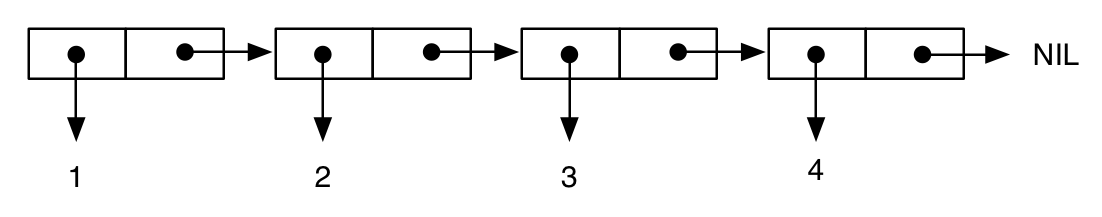
\includegraphics[width=\linewidth]{../img/cons.png}
  \caption{Cons cells forming a list\autocite{cons-image-source}}
  \label{fig:cons}
\end{figure}

The cons operator thus prepends an element to a list, effectively allocating a
variable that contains the newly added element and a pointer to the `old' list.
As a result, prepending to a list is computationally cheap, needing one allocation
and one update.

In Haskell, the `name' of the cons function is the `:' operator.
In Go, names for identifiers (which includes function names) underlie a simple
rule:
\begin{quote}
    An identifier is a sequence of one or more letters and digits. The first
    character in an identifier must be a letter.\autocite{spec-identifiers}
\end{quote}

This rule forbids a function to be named `:'. Instead, the function could be
named `cons'. However, Go already has a function to add to the end of a slice,
`append'. Thus, adding to the beginning of a slice will be named `prepend'.
Using prepend is very similar to append, an example can be found at~\ref{code:prepend-go}

\begin{code}
    \captionof{listing}{Example usage of prepend in go}
    \label{code:prepend-go}
    \begin{gocode}
package main

import (
        "fmt"
        "strconv"
)

func main() {
        fmt.Printf("%#v", prepend(0, []int{1, 2, 3}))
}
\end{gocode}
\begin{bashcode}
$> fgo run .
[]int{0, 1, 2, 3}
\end{bashcode}
\end{code}

\subsection{Fold}\label{sec:fold}

Fold, sometimes also named `reduce' or `aggregate' is another higher-order function
that is very commonly used in functional programming.

\begin{quote}
    analyze a recursive data structure and through use of a given
    combining operation, recombine the results of recursively processing its
    constituent parts, building up a return value.\autocite{fold-wiki}
\end{quote}

The family of fold functions in Haskell consist of three different implementations of
that definition: `foldr', `foldl' and `foldl\''.
The difference between foldr and foldl is hinted at their function headers:
\begin{code}
    \captionof{listing}{Function headers of the fold functions}
    \begin{haskellcode}
Prelude Data.List> :t foldr
foldr :: Foldable t => (a -> b -> b) -> b -> t a -> b
Prelude Data.List> :t foldl
foldl :: Foldable t => (b -> a -> b) -> b -> t a -> b
    \end{haskellcode}
\end{code}

The argument with type `b' is passed as the first argument to the foldl
function, and as the second argument to foldr. As can be seen in the illustrations
of foldl and foldr in~\ref{fig:fold}, the evaluation order of the two functions
differ.

\begin{figure}[h!]
    \centering
    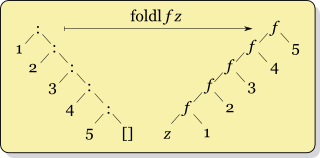
\includegraphics[scale=0.5]{../img/foldl.png}
    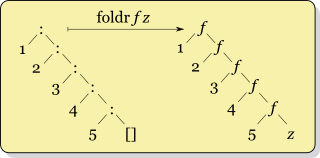
\includegraphics[scale=0.5]{../img/foldr.png}
    \caption{Folds illustrated\autocite{fold-wiki}}
    \label{fig:fold}
\end{figure}

This is most obvious when using an example where the function is not associative:

\begin{code}
    \captionof{listing}{foldr and foldl execution order}
    \label{code:foldr-example}
    \begin{haskellcode}
foldr (-) 0 [1..7]
1 - (2 - (3 - (4 - (5 - (6 - (7 - 0)))))) = 4
foldl (-) 0 [1..7]
((((((0 - 1) - 2) - 3) - 4) - 5) - 6) - 7 = -28
    \end{haskellcode}
\end{code}

In foldl, the accumulator (`0') is added to the left end of the list (prepended),
while with foldr, the accumulator is added to the right end.
For associative functions (e.g. `+') this does not make a difference, it does
however for non-associative functions, as can be seen in the example~\ref{code:foldr-example}.

The difference between foldl and foldl' is more subtle:
\begin{quote}
    foldl and foldl' are the same except for their strictness properties, so if both
    return a result, it must be the same.\autocite{fold-types}
\end{quote}

The strictness property is only relevant if the function is lazy in its first argument,
meaning that foldl builds up an execution path, while foldl' executes the instructions
while traversing it:

\begin{code}
    \captionof{listing}{foldl and foldl' strictness\autocite{fold-types}}
    \begin{haskellcode}
> (?) :: Int -> Int -> Int
> _ ? 0 = 0
> x ? y = x*y
>
> list :: [Int]
> list = [2,3,undefined,5,0]
>
> foldl (?) 1 list
foldl (?) 1 [2,3,undefined,5,0] -->
foldl (?) (1 ? 2) [3,undefined,5,0] -->
foldl (?) ((1 ? 2) ? 3) [undefined,5,0] -->
foldl (?) (((1 ? 2) ? 3) ? undefined) [5,0] -->
foldl (?) ((((1 ? 2) ? 3) ? undefined) ? 5) [0] -->
foldl (?) (((((1 ? 2) ? 3) ? undefined) ? 5) ? 0) [] -->
((((1 ? 2) ? 3) ? undefined) ? 5) ? 0 -->
0

> foldl' (?) 1 list
foldl' (?) 1 [2,3,undefined,5,0] -->
    1 ? 2 --> 2
foldl' (?) 2 [3,undefined,5,0] -->
    2 ? 3 --> 6
foldl' (?) 6 [undefined,5,0] -->
    6 ? undefined -->
*** Exception: Prelude.undefined
    \end{haskellcode}
\end{code}

To keep things simpler, Go will only have its versions of foldl and foldr, which
will both be strict - the Haskell counterparts would thus be foldr and foldl'.\footnote{
If the behaviour from the normal foldl function is required, a workaround can
be applied in th Go version. See appendix~\ref{appendix:foldl-go}
}
The usage of these fold-functions is equal to the Haskell versions, where foldl's
arguments are switched in order.

\begin{code}
    \captionof{listing}{Example usage of foldr and foldl in go}
    \label{code:fold-go}
\begin{gocode}
package main

import "fmt"

func main() {
        fmt.Printf("%v\n", foldr(func(x, y int) int { return x - y }, 100, []int{10, 20, 30}))
        fmt.Printf("%v\n", foldl(func(x, y int) int { return x - y }, 100, []int{10, 20, 30}))
}
\end{gocode}
\begin{bashcode}
$> fgo run .
-80
40
\end{bashcode}
\end{code}

\section{Functional Check}


\chapter{Implementation}
\label{ch:implementation} % chktex 24
\section{Implementing the new built-in functions}

\subsection{Required Steps}

Adding a builtin function to the Go language requires a few more steps than just
adding support within the compiler. While it would technically be enough to
support the translation between Go code and the compiled binary, there would be
no visibility for a developer that there is a function that could be used.
For a complete implementation, the following steps are necessary:
\begin{itemize}
    \item Adding the GoDoc\autocite{godoc} that describes the function and it's usage
    \item Adding type-checking support in external packages for tools like
        Gopls\footnote{Gopls is Go's official language server implementation\autocite{gopls}.}
    \item Adding the implementation within the internal\footnote{
            ``An import of
            a path containing the element “internal” is disallowed if the
            importing code is outside the tree rooted at the parent of the
            `internal' directory.''\autocite{internal-packages}
        }
        package of the compiler
        \begin{itemize}
            \item Adding the \gls{ast} node type
            \item Adding type-checking for that node type
            \item Adding the AST traversal for that node type, translating it
                to AST nodes that the compiler already knows and can translate
                to builtin runtime-calls or \gls{ssa}
        \end{itemize}
\end{itemize}

The Go source code that is relevant for this thesis can be classified into three different
types. One is the godoc - the documentation for the new built-in functions. The
other two are the `public' and the `private' implementation of these builtins.

The `private' implementation is located within the
\textit{src/cmd/compile/internal} package\autocite{internal-packages}. It can only
be used by the package in \textit{src/cmd/compile}, which contains the
implementation of the compiler itself.

When calling \mintinline{shell}|go build .|, the compiler is invoked indirectly
through the main `go' binary. To directly invoke the compiler,
\mintinline{shell}|go tool compile| can be used.

Everything that is not in \textit{src/cmd/compile} is referred to as the `public'
part of the compiler in this thesis. The `public' parts are used by external
tools, for example Gopls, for type-checking, source code validation and
analysis.

\subsection{Adding the GoDoc}
In Go, documentation is generated directly from comments within the source code
\autocite{godoc}. This also applies to builtin functions in the compiler, which
have a function stub to document their behaviour\autocite{godoc-builtin}, but
no implementation, as that is done in the compiler\autocite{builtin-impl}.

The documentation for builtins should be as short and precise as possible.
The usage of `Type' and `Type1' has been decided based on other builtins
like `append' and 'delete'.
The function headers are derived from their Haskell counterparts, adjusted
to the Go nomenclature.

\begin{code}
    \captionof{listing}{Godoc for the new built-in functions}
    \gofilerange{../work/go/src/builtin/builtin.go}{begin-newbuiltins}{end-newbuiltins}
\end{code}
\subsection{Public packages}

\begin{quote}
Note that the `go/*` family of packages, such as `go/parser` and `go/types`,
have no relation to the compiler. Since the compiler was initially written in C,
the `go/*` packages were developed to enable writing tools working with Go code,
such as `gofmt` and `vet`.\autocite{compiler-readme}
\end{quote}

To enable tooling support for the new built-in functions, they have to be
registered in the `go/*' packages. The only package that is affected by new
builtins is `go/types'.

In the `types' package, the builtins have to be registered as such and as
`predeclared' functions:

\begin{code}
    \captionof{listing}{Registering new built-in functions}
    \gofilerange{../work/go/src/go/types/universe.go}{start-builtin}{end-builtin}
    \gofilerange{../work/go/src/go/types/universe.go}{start-predeclared}{end-predeclared}
\end{code}
This registration defines the type of the built-in - they are all expressions,
as they return a value - and the number of arguments.
After that, the type-checking and its associated tests are to be implemented.

This concludes the type-checking for external tools and makes `gopls' return errors
Once type-checking the new built-in functions is implemented, `gopls' can be
compiled against the new public packages.\footnote{
This means pointing the Go toolchain to the correct directory by setting
the value of `GOROOT' with \mintinline{shell}|go env -w GOROOT=<path>|.
}
It will then return errors if the wrong types are used. For example, when trying
to prepend an integer to a string slice:

\begin{gocode}
package main

import "fmt"

func main() {
    fmt.Println(prepend(3, []string{"hello", "world"}))
}
\end{gocode}

Gopls will report a type-checking error:
\begin{bashcode}
$ gopls check main.go
/tmp/playground/main.go:6:22-23: cannot convert 3 (untyped int constant) to string
\end{bashcode}

\subsection{Private packages}

In the private packages - the actual compiler - the expressions have to be
type-checked, ordered and transformed.

The type-checking process is similar to the one executed for external tools.
It should also check the node's child nodes, meaning an operations
arguments, body and init statements. Furthermore, during the type-checking
process, the built-in function's return types are set and node types
may be converted, if possible and necessary.
An operation may expect it's arguments to be in \mintinline{go}|node.Left|
and \mintinline{go}|node.Right|, which means type-checking will also need
to move the argument nodes from their default location in
\mintinline{go}|node.List| to \mintinline{go}|node.Left| and
\mintinline{go}|node.Right|.

Ordering ensures the evaluation order and re-orders expressions. All of
the new built-in functions will be evaluated left-to-right and there are now
special cases to handle.

Transforming means changing the AST nodes from the built-in operation to
nodes that the compiler knows how to translate to SSA. The actual algorithm
that these functions use cannot be implemented in normal Go code, they have to be
translated directly to AST nodes and statements.

There are more steps to compiling Go code, for example escape-checking,
SSA conversion and a lot of optimisations. These are not necessary to
implement and do not have a direct relation to the new built-ins, which
is why these steps are elided in this paper.

The actual algorithms and part of the implementations for the builtin
functions are covered in the following chapters.
\footnote{
    The full implementations can be viewed by diff-ing the git repository
    between the references `bachelor-thesis' and `go1.14'\autocite{ba-go1-14-thesis-diff}.
}

\subsubsection{fmap}\label{ch:impl-fmap}

To make the implementation in the AST easier, the algorithm will first be
developed in Go, and then translated. Implementing fmap in Go is relatively
simple:

\begin{code}
    \captionof{listing}{Fmap implementation in Go}
    \label{code:fmap-go}
    \begin{gocode}
func fmap(fn func(Type) Type1, src []Type) (dest []Type1) {
    for _, elem := range src {
        dest = append(dest, fn(elem))
    }
    return dest
}
\end{gocode}
\end{code}
However, there is room for improvement within that function. Instead
of calling \mintinline{go}|append| at every iteration of the loop, the slice can
be allocated with \mintinline{go}|make| at the beginning of the function. Thus,
calls to grow the slice at runtime can be saved.

\begin{code}
    \captionof{listing}{Improved implementation of fmap}
    \label{code:fmap-go-improved}
    \begin{gocode}
func fmap(fn func(Type) Type1, src []Type) []Type1 {
    dest := make([]Type1, len(src))
    for i, elem := range src {
        dest[i] = fn(elem)
    }
    return dest
}
    \end{gocode}
\end{code}
This algorithm can be translated to the following AST node:

\begin{code}
    \captionof{listing}{fmap AST translation\autocite{fmap-walk-implementation}}
    \gofilerange{../work/go/src/cmd/compile/internal/gc/walk.go}{start-fmap-header}{end-fmap-header}
\end{code}
\subsubsection{prepend}

The general algorithm for `prepend' is:
\begin{code}
    \captionof{listing}{prepend implementation in Go}
    \begin{gocode}
func prepend(elem Type, slice []Type) []Type {
    dest := make([]Type, 1, len(src)+1)
    dest[0] = elem
    return append(dest, slice...)
}
    \end{gocode}
\end{code}
The call to \mintinline{go}|make(...)| creates a slice with the length of 1 and the capacity
to hold all elements of the source slice, plus one. By allocating the slice with the full
length, another slice allocation within the call to \mintinline{go}|append(...)| is saved.
The element to prepend is added as the first element of the slice, and append will then
copy the `src' slice into `dest'.

The implementation within `walkprepend' reflects these lines of Go code, but
as AST nodes:

\begin{code}
    \captionof{listing}{prepend AST translation\autocite{prepend-walk-implementation}}
    \gofilerange{../work/go/src/cmd/compile/internal/gc/walk.go}{start-prepend-header}{end-prepend-header}
\end{code}
\subsubsection{foldr and foldl}

As outlined in Chapter~\ref{sec:fold}, there will be two fold functions;
foldr and foldl. foldr behaves exactly like its Haskell counterpart,
while foldl behaves like foldl' in Haskell.

While the fold algorithms are most obvious when using recursion, due to
performance considerations, an imperative implementation has been chosen:

\begin{code}
    \captionof{listing}{fold implementation in Go}
    \begin{gocode}
func foldr(fn func(Type, Type1) Type1, acc Type1, slice []Type) Type1 {
    for i := len(s) - 1; i >= 0; i-- {
        acc = fn(s[i], acc)
    }
    return acc
}

func foldl(fn func(Type1, Type) Type1, acc Type1, slice []Type) Type1 {
    for i := 0; i < len(s); i++ {
        acc = f(acc, s[i])
    }
    return acc
}
\end{gocode}
\end{code}
The code further clarifies the differences between the two different folds;
the slice is processed in reverse order for foldr (as it would be if this
algorithm would have been implemented with recursion), and the order of
arguments to the fold function is switched.

The AST walk translates fold to:
\begin{code}
    \captionof{listing}{fold AST translation\autocite{fold-walk-implementation}}
    \gofilerange{../work/go/src/cmd/compile/internal/gc/walk.go}{start-fold-header}{end-fold-header}
\end{code}
\subsubsection{filter}\label{ch:impl-filter}

Being a slice-manipulating function, filter also needs to traverse the whole
slice in a for-loop. However, compared to the other newly built-in functions,
the size for the target slice is unknown until all items have been traversed,
which is why filter does not allow for the same optimisations as the other
functions.

\begin{code}
    \captionof{listing}{filter implementation in Go}
    \begin{gocode}
func filter(f func(Type) bool, s []Type) []Type {
    var dst []Type
    for i := range s {
            if f(s) {
                dst = append(dst, s[i])
            }
    }
}
    \end{gocode}
\end{code}
And the same algorithm, but translated to AST statements:

\begin{code}
    \captionof{listing}{filter AST translation\autocite{filter-walk-implementation}}
    \gofilerange{../work/go/src/cmd/compile/internal/gc/walk.go}{start-filter-header}{end-filter-header}
\end{code}


\clearpage
\section{Functional Check}
As discussed in Chapter~\ref{sec:funcheck-theory}, to assist writing purely
functional code, a linter needs to be written that detects reassignments within
a Go program.

To get a grasp about the issues this linter should report, the first step
is to capture some examples, cases that should be matched against.

\subsection{Examples}

The simplest cases are standalone reassignments and assignment operators:
\begin{gocode}
x := 5
x = 6 // forbidden
// or
var y = 5
y = 6   // forbidden
y += 6  // forbidden
y <<= 2 // forbidden
y++     // forbidden
\end{gocode}

Where the statements with a \mintinline{go}|// forbidden
| comment should be reported.

Adding block scoping to this, shadowing the old variable needs to be allowed:
\begin{gocode}
x := 5
{
	x = 6  // forbidden, changing the old value
	x := 6 // allowed, as this shadows the old variable
}
\end{gocode}

What should be illegal is to declare the variable first and then assign a
value to it:
\begin{gocode}
var x int
x = 6 // forbidden
\end{gocode}

The exception here are functions, as they need to be declared first in order
to recursively call them:
\begin{gocode}
var f func()
f = func() {
	f()
}
\end{gocode}

Furthermore, the linter also needs to be able to handle multiple variables
at once:
\begin{gocode}
var f func()
x, f, y := 1, func() { f() }, 2
\end{gocode}

Loops should be reported too, as they are using reassignments internally:
\begin{gocode}
for i := 0; i < 5; i++ { // forbidden
	for i != 3 { // forbidden
		for { // allowed
			// ...
		}
	}
}
\end{gocode}

All the aforementioned examples and more can be found in the testcases for funcheck\autocite{funcheck-examples}.

\subsection{Building a linter}

The Go ecosystem already provides an official library for building code analysis tools,
the `analysis' package from the Go Tools repository\autocite{go-analysis}. With this package,
implementing a static code analyser is being reduced to writing the actual AST node analysis.

To define an analysis, a variable of type \mintinline{go}|*analysis.Analyzer| has to be declared:

\begin{gocode}
var Analyzer = &analysis.Analyzer{
	Name: "assigncheck",
	Doc:  "reports reassignments",
	Run:  func(*analysis.Pass) (interface{}, error)
}
\end{gocode}

The necessary steps are now adding the `Run' function and registering the analyser
in the \mintinline{go}|main()| function.

The `Run' function takes an \mintinline{go}|*analysis.Pass| type. The Pass provides
information about the package that is being analysed and some helper-functions to report
diagnostics.

With `analysis.Pass.Files` and the help of the `go/ast` package, traversing the syntax
tree of every file in a package is made extremely convenient:

\begin{gocode}
for _, file := range pass.Files {
	ast.Inspect(file, func(n ast.Node) bool {
		// node analysis here
	})
}
\end{gocode}

To implement funcheck as described, five different AST node types need to be
taken care of. The simpler ones are
\mintinline{go}|*ast.IncDecStmt|, \mintinline{go}|*ast.ForStmt| and \mintinline{go}|*ast.RangeStmt|.
An `IncDecStmt' node is a \mintinline{go}|x++| or \mintinline{go}|x--|
expression and should always be reported.
`ForStmt' and `RangeStmt' are similar; a `RangeStmt' is a `for' loop with the
\mintinline{go}|range| keyword instead of an init-, condition- and post-stametent.

Both of these loop-types need to be reported explicitly as they do not show up
as reassignments in the AST.
The basic building blocks for our is the following \mintinline{go}|switch|
statement:
\begin{code}
	\gofilerange{../work/funcheck/assigncheck/assigncheck.go}{start-basictypes}{end-basictypes}
	\caption{Handling the basic AST types in funcheck}
\end{code}
The remaining two node types are \mintinline{go}|*ast.DeclStmt| and \mintinline{go}|*ast.AssignStmt|.
They are not as simple to handle, which is why they are covered in their own chapters.

\subsection{Detecting reassignments}

To recapitulate, the goal of this step is to detect all assignments except blank identifiers
(discarded values cannot be mutated) and function literals, if the function is declared in the
last statement\footnote{This rule is to simplify the logic of the checker and make it easier
    for developers to read the code. It means that no code may be between \mintinline{go}|var f func|
and \mintinline{go}|f = func() { ... }|.}.

To detect such reassignments, funcheck iterates over all identifiers on the left-hand side
of an assignment statement.

On the left-hand side of an assignment is a list of expressions. These expressions can be
identifiers, index expressions (\mintinline{go}|*ast.IndexExpr|, for map and slice access),
a `star expression' (\mintinline{go}|*ast.StarExpr|\footnote{star expressions
    are expressions that are prefixed by an asterisk, dereferencing a pointer. For example
\mintinline{go}|*x = 5|, if \mintinline{go}|x| is of type \mintinline{go}|*int|.}) or others.

If the expression is not an identifier, the assignment must be a reassignment, as all non-identifier
expressions contain an already declared identifier. For example, the slice index expression
\mintinline{go}|s[5]| is of type \mintinline{go}|*ast.IndexExpr|:
\begin{gocode}
// An IndexExpr node represents an expression followed by an index.
IndexExpr struct {
	X      Expr      // expression
	Lbrack token.Pos // position of "["
	Index  Expr      // index expression
	Rbrack token.Pos // position of "]"
}
\end{gocode}

Where \mintinline{go}|IndexExpr.X| is our identifier `s' (of type \mintinline{go}|*ast.Ident|)
and a \mintinline{go}|IndexExpr.Index| is \mintinline{go}|5| (of type \mintinline{go}|*ast.BasicLit|).

As these nested identifiers already need to be declared beforehand (else they could not be used
in the expression), all expressions on the left-hand side of an assignment that are not identifiers
are reassignments.

Identifiers are the only expressions that can occur in declarations and reassignments. A naive
approach would be to check for the colon in a short variable declaration (\mintinline{go}|:=|).
However, as touched upon in Chapter~\ref{sec:multi-assign}, even short variable declarations may
contain redeclarations, if at least one variable is new.

Thus, another approach is needed.

Every identifier (an AST node with type \mintinline{go}|*ast.Ident|) contains an object\footnote{`An
    object describes a named language entity such as a package, constant, type, variable,
function (incl. methods), or a label'\autocite{go-ast-object}.} that links to the declaration.

This declaration, of whatever type it may be, always has a position (and a corresponding function
to retrieve that position) in the source file.

A reassignment is detected if an identifier's declaration position does not match the assignment's
position (indicating that the variable is being assigned at a different place to where it is
declared).

This is illustrated in the code block~\ref{code:assign-pos}. What can be clearly seen is that in
the assignment \mintinline{go}|y = 3|, \mintinline{go}|y|'s declaration refers to the position
of the first assignment \mintinline{go}|x, y := 1, 2|, the position where \mintinline{go}|y| has
been declared.
\begin{listing}
    \begin{gocode}
Assignment "x, y := 1, 2": 2958101
        Ident "x": 2958101
                Decl "x, y := 1, 2": 2958101
        Ident "y": 2958104
                Decl "x, y := 1, 2": 2958101
Assignment "y = 3": 2958115
        Ident "y": 2958115
                Decl "x, y := 1, 2": 2958101
    \end{gocode}
\caption{Illustration of an assignment node and corresponding positions\autocite{ast-positions}\label{code:assign-pos}}
\end{listing}

As this technique works on an identifier level, multi-variable declarations or assignments
can be verified without any additional effort.

If a variable in a short variable declaration is being reassigned, the variable's `Declaration'
field will point to the original position of its declaration, which can be easily detected
(as shown in code block~\ref{code:assign-pos}).

\subsection{Handling function declarations}

In contrast to all other variable types, function variables may be `reassigned' once.
As discussed in Chapter~\ref{sec:func-reassign}, this is to allow recursive function
literals. Detecting and not reporting these assignments is a two-step process, as two
consecutive AST nodes need to be inspected.

The first step is to detect function declarations; statements of the form
\mintinline{go}|var f func() |. Should such a statement be encountered,
its position is saved for the following AST node.

In the consecutive AST node it is ensured that, if the node is an assignment and
the assignee identifier is of type function literal, the position matches the
previously saved one.

The position of the declaration and AST node structure can be seen in~\ref{code:func-reassign}

\begin{listing}
    \begin{gocode}
Declaration "var f func() int": 2958142
        Ident "f func() int": 2958146
Assignment "f = func() int { return y }": 2958160
        Ident "f": 2958160
                Decl "f func() int": 2958146
\end{gocode}
	\caption{Illustration of a function literal assignment\autocite{ast-positions}\label{code:func-reassign}}
\end{listing}

With this technique it is possible to exempt functions from the reassignment rule.

\subsection{Testing Funcheck}

The analysis-package is distributed with a sub-package `analysistest'. This package makes
it extremely simple to test a code analysis tool.

By providing test data and the expected messages from funcheck in a structured way, all
that is needed to test funcheck is:

\begin{code}
\begin{gocode}
package assigncheck

import (
        "testing"

        "golang.org/x/tools/go/analysis/analysistest"
)

func TestRun(t *testing.T) {
        analysistest.Run(t, analysistest.TestData(), Analyzer)
}
\end{gocode}
    \caption{Testing a code analyser with the `analysistest' package}
\end{code}

The library expects the test data in the current directory in a folder named `testdata' and
then spawns and executes the analyser on the files in that folder. Comments in those files
are used to describe the expected message:

\begin{gocode}
x := 5
fmt.Println(x)
x = 6 // want `^reassignment of x$`
fmt.Println(x)
\end{gocode}

This will ensure that on the line \mintinline{go}|x = 6| an error message is reported that says
`reassignment of x'.



\chapter{Application}
\label{ch:application} % chktex 24
% -*- mode: latex; coding: utf-8; TeX-master: ../thesis -*-
% !TEX TS-program = pdflatexmk
% !TEX encoding = UTF-8 Unicode
% !TEX root = ../thesis.tex

\section{Refactoring the Prettyprint Package}

\newglossaryentry{stdout}{name=stdout, description={Standard Output, the default
output stream for programs}}

The code blocks~\ref{code:assign-pos} and~\ref{code:func-reassign} have been
generated by a small package `prettyprint' contained in the funcheck repository.

To see how the newly built-in functions and funcheck can be used, this `prettyprint' package
can be refactored to a purely functional version.
The current version of the package is written in what could be considered idiomatic
Go\footnote{
	There is no exact definition of what idiomatic Go is, so this interpretation
	could be challenged. It is idiomatic Go code to the author of this thesis.
}. %TODO?


The prettyprinter is based on the same framework as assigncheck\footnote{Assigncheck
is the main package for funcheck and checks the reassignments}, but instead
of reporting anything, it prints AST information to \gls{stdout}.

Similarly to assigncheck, the main logic of the package is within a
function literal that is being passed to the \mintinline{go}|ast.Inspect|
function.

Prettyprint only checks two AST node types, \mintinline{go}|*ast.DeclStmt|
and \mintinline{go}|*ast.AssignStmt| (declarations and assignments).

For example, for the program
\begin{gocode}
package main

import "fmt"

func main() {
	x, y := 1, 2
	y = 3
	fmt.Println(x, y)
}
\end{gocode}
the following AST information is printed:

\begin{gocode}
Assignment "x, y := 1, 2": 2958101
		Ident "x": 2958101
				Decl "x, y := 1, 2": 2958101
		Ident "y": 2958104
				Decl "x, y := 1, 2": 2958101
Assignment "y = 3": 2958115
		Ident "y": 2958115
				Decl "x, y := 1, 2": 2958101
\end{gocode}

To refactor it to a purely functional version, funcheck can be used to
list reassignments:

\begin{bashcode}
$> funcheck .
prettyprint.go:20:2: internal reassignment (for loop) in "for _, file := range pass.Files { ... }"
prettyprint.go:42:2: internal reassignment (for loop) in "for i := range decl.Specs { ... }"
prettyprint.go:67:2: internal reassignment (for loop) in "for _, expr := range as.Lhs { ... }"
\end{bashcode}
As can be seen in the output, the package uses 3 \mintinline{go}|for| loops to range over
slices. However, there are no other reassignments of variables in the code.

The code to print declarations, which causes the second lint message, is as shown in~\ref{code:decl-printing}.

\begin{code}
\begin{gocode}
func checkDecl(as *ast.DeclStmt, fset *token.FileSet) {
	fmt.Printf("Declaration %q: %v\n", render(fset, as), as.Pos())
	decl, ok := as.Decl.(*ast.GenDecl)
	if !ok {
		return
	}

	for i := range decl.Specs {
		val, ok := decl.Specs[i].(*ast.ValueSpec)
		if !ok {
			continue
		}

		if val.Values != nil {
			continue
		}

		if _, ok := val.Type.(*ast.FuncType); !ok {
			continue
		}

		fmt.Printf("\tIdent %q: %v\n", render(fset, val), val.Names[0].Pos())
	}
}
\end{gocode}
	\caption{Pretty-printing declarations in idiomatic Go\label{code:decl-printing}}
\end{code}
To convert this for-loop appropriately, the new built-in `foldl' can be used.
To recapitulate, the `foldl' function is being defined as:
\begin{gocode}
func foldl(fn func(Type1, Type) Type1, acc Type1, slice []Type) Type1
\end{gocode}
As `foldl' requires a return type, a dummy type `null" can be introduced, which
is just an empty struct:
\begin{gocode}
type null struct{}
\end{gocode}
Now the code within the foor loop can be used to create a function literal:
\begin{gocode}
check := func(_ null, spec ast.Spec) (n null) {
	// implementation
}
\end{gocode}
There are two subtleties in regards to the introduced null type:
First, the null value that is being passed as an argument is being discarded
by the use of an empty identifier.
Secondly, the return value is `named', which means the variable `n' is
already declared in the function block. Because of this, `naked returns' can
be used, so there is no need to specify which variable is being returned.

The snippet~\ref{code:decl-printing} can be translated to

\begin{code}
	\begin{gocode}
func checkDecl(as *ast.DeclStmt, fset *token.FileSet) {
	fmt.Printf("Declaration %q: %v\n", render(fset, as), as.Pos())

	check := func(_ null, spec ast.Spec) (n null) {
		val, ok := spec.(*ast.ValueSpec)
		if !ok {
			return
		}

		if val.Values != nil {
			return
		}

		if _, ok := val.Type.(*ast.FuncType); !ok {
			return
		}

		fmt.Printf("\tIdent %q: %v\n", render(fset, val), val.Names[0].Pos())
		return
	}

	if decl, ok := as.Decl.(*ast.GenDecl); ok {
		_ = foldl(check, null{}, decl.Specs)
	}
}
\end{gocode}
	\caption{Pretty-printing declarations in functional Go}
\end{code}
The for-loop has been replaced by a `foldl', where a function closure
that contains the actual processing is passed.

While this still looks similar to the original example, this is mostly due to
the `if' statements. In Haskell, pattern matching would be used and nil checks
could be omitted entirely. Also, as Haskell's type system is more advanced, the
handling of those types would be different too.

However, the goal of this thesis is to make functional code look more familiar
to programmers that are used to imperative code.
And while it may not look like it, the code does not use any mutation of
variables\footnote{Libraries may do, but the scope is not to rewrite any existing
libraries.}, for loops or global state. Therefore, it can be concluded that this
snippet is purely functional as per the definition from Chapter~\ref{sec:func-purity}.

\section{Quicksort}

In Chapter~\ref{code:haskell-quicksort}, a naive implementation of the Quicksort sorting
algorithm has been introduced.
Implementing this algorithm in Go is now straightforward and the similarities between
the Haskell implementation and the functional Go implementation are striking:

\begin{listing}
	\begin{gocode}
func quicksort(p []int) []int {
	if len(p) == 0 {
		return []int{}
	}

	lesser := filter(func(x int) bool { return p[0] > x }, p[1:])
	greater := filter(func(x int) bool { return p[0] <= x }, p[1:])

	return append(quicksort(lesser), prepend(p[0], quicksort(greater))...)
}
\end{gocode}
\begin{haskellcode}
quicksort :: Ord a => [a] -> [a]
quicksort []     = []
quicksort (p:xs) = (quicksort lesser) ++ [p] ++ (quicksort greater)
    where
        lesser  = filter (< p) xs
        greater = filter (>= p) xs
\end{haskellcode}
	\caption{Quicksort implementations compared}
\end{listing}

Again, the Go implementation bridges the gap between being imperative and functional,
while still being obvious about the algorithm.
Furthermore, as expected, when inspecting the code with funcheck, no non-functional
constructs are reported.

\section{Comparison to Java Streams}

In Java 8, concepts from functional programming have been introduced to the language.
The major new feature was Lambda Expressions --- anonymous function literals --- and
streams. Streams are an abstract layer to process data in a functional way, with `map',
`filter', `reduce' and more.

Java Streams are similar to the new built-in functions in this thesis:

\begin{listing}
	\begin{javacode}
List<Integer> even = list.stream()
	.filter(x -> x % 2 == 0)
	.collect(Collectors.toList());
	\end{javacode}
	\begin{gocode}
even := filter(
	func(x int) bool { return x%2 == 0 },
	list)
	\end{gocode}
	\caption{Comparison Java Streams and functional Go}
\end{listing}

The lambda-syntax in Java is more concise than Go's function literals, where the
complete function header has to be provided\footnote{There is an open proposal
	to add a lightweight anonymous function syntax to Go 2, which, if implemented,
would resolve this verbosity\autocite{go-lambdas}}.
%Before lambdas have been introduced in Java 8, the way to achieve this was through
%anonymous inner classes. This means that due to the historic growth of Java, there
%are currently two methods to define an anonymous functions, which may cause inconsistencies
%in the code. However, anonymous inner classes are extremely verbose if the goal is
%to introduce only one function\autocite{java-lambda-expressions}:

%\begin{javacode}
%printPersons(
	%roster,
	%new CheckPerson() {
		%public boolean test(Person p) {
			%return p.getGender() == Person.Sex.MALE
				%&& p.getAge() >= 18
				%&& p.getAge() <= 25;
		%}
	%}
%);
%\end{javacode}

%Already because of the overhead in typing, most programmers will prefer to use
%lambdas.
%%If this is used, Go's function literal syntax has an edge over Java's when it comes to
%%readability and conciseness.

% TODO: Is this really about only one list type?
However, the conversion to a stream and back to a list (with \mintinline{java}|list.stream()| and
\mintinline{java}|.collect(Collectors.toList())|)
is not required in Go, as the operations all work on slices. Here, only having a single
list-like type built into the language is an advantage, as the (at least syntactical)
overhead to convert the list only to run a `filter' function can be avoided.

Apart from syntactical differences, Java Streams contain all the functions that
have been added as built-ins to Go too, and a lot more.

On the other hand, Java's Syntax is arguably more complex than Go. An indicator for this might be
the language specification; Go's Language Specification is roughly 110 pages, while
Java's specification spans more than 700 pages\footnote{
	The Java 8 Specification is 724\autocite{java-8-spec}, the Java 14
	Specification 774\autocite{java-14-spec} pages.}, more than 6 times the size.

The consideration of which language to choose comes down to the experience with either language.
An experienced Java programmer will find it easier to start with Java's toolset, while programmers
coming from a C background may choose Go over Java.


\IfLanguageName{nswissgerman}{\chapter{Resultate}}{\chapter{Results}}
\label{ch:results} % chktex 24
% -*- mode: latex; coding: utf-8; TeX-master: ../thesis -*-
% !TEX TS-program = pdflatexmk
% !TEX encoding = UTF-8 Unicode
% !TEX root = ../thesis.tex

To learn functional programming without being introduced to a new syntax at the same time
ensures that programmers can fully concentrate on functional concepts. Although Go already
supported a functional programming style, the programmer may not have known if the code is
purely functional or if there are still imperative constructs embedded.

In the last chapters, functional purity has been defined as a law based on two rules; immutability
and function purity. Immutability means that once assigned, a variable's value never
changes. Function purity entails that functions do not have side effects and their return
value is solely influenced by the function's parameters.

It has been shown that although purely functional languages like Haskell aim to be completely
pure, this objective is difficult to accomplish. The reason for this are Input / Output actions; user
input, network connections, randomness and time are all impure. Haskell wraps
these impure functions in the IO monad, which is a way to work around the compiler's optimisations
based on functional purity. While the IO monad does not make impure functions pure, it
does serve as documentation to it's users (`if the function has IO, it is impure') and
guarantees a certain execution order.

Go on the other hand does not have this issue. The Go compiler does not optimise execution
based on purity guarantees. Having a similar construct like the IO monad in Go would as such
only serve documentation purposes. Because of this, the decision has been taken to ignore
the impurity that is implied with IO actions.

Apart from IO, to achieve functional purity, the global state of a program should not influence
the return values of specific function. This ties into immutablitiy; if global state can
not be mutated, it can also not influence or change the result value of a function.

Based on these observations, a static code analysis tool has been developed that reports
all reassignments of variables. In other words, it forbids the usage of the regular
assignment operator (\mintinline{go}|=|), only allowing the short variable declarations
(\mintinline{go}|:=|). However, the experienced Go developer may know that the \mintinline{go}|:=|
operator can also reassign previously declared variables, implying that the solution to the
problem is not as simple as forbidding the assignment operator.
Further, there are many more edge cases that have been detected with careful testing:
To recursively call function literals, they must be declared beforehand (before assigning
the actual function to it) because of Go's scoping rules. Additionally, exceptions
had to be made for the blank identifier (\mintinline{go}|_|) and variables that are declared
outside of the current file.

With all of this in place, an algorithm has been chosen that is based on the identifier's
declaration position. In the \gls{ast} that is being checked, every identifier node has a field
which contains the position of it's declaration. If this does not match the current identifier's
position, the operation must be a reassignment.
The resulting binary, called `funcheck', successfully reports such reassignments:

\begin{gocode}
s := "hello world"
fmt.Println(s)
s = "and goodbye"
fmt.Println(s)
\end{gocode}

\begin{bashcode}
\$> funcheck .
file.go:3:2: reassignment of s
\end{bashcode}

This linter can be used and ran against any Go package. To eliminate the reported errors,
code has to be rewritten in what ends up being purely functional code.

However, functional code often relies heavily on lists and list-processing functions.
Although Go does not have a built-in list datatype, Go's slices, an abstraction on arrays,
mitigate a lot of downsides when comparing regular arrays to lists\footnote{Arrays / Slices
and Lists have a completely different runtime behaviour (indexing, adding or removing elements).
However, the performance of the code was not considered to be relevant in this thesis.}.

What Go's slices lack on the other side are the typical higher-order functions like `map',
`filter' or `reduce'. These are commonly used in functional programming and most languages
contain implementations of these functions already --- Go does not.

Due to the lack of polymorphism, writing implementations for these functions
would result in a lot of duplicated code. To mitigate this issue, the most
common higher-order functions have been added to the list of Go's built-in functions,
which are registered, type-checked and implemented within the Go compiler.
As these are handled directly at compile time, built-in functions may be polymorphic, for
example allowing the programmer to use the same `filter' function for all list-types.

To determine which higher-order functions are most commonly used, we analysed the most
popular open-source Haskell projects (pandoc, shellcheck and purescript, to name a few).
As a result, `fmap', `fold', `filter' and `prepend'
(`cons') have been added as built-ins into the compiler.
These functions make it easier to write purely functional code in Go, in turn helping
the programmer to learn functional programming with a familiar language and syntax.

While implementing these functions in a regular Go program would be a matter of minutes,
adding them to the Go compiler is more effort. To illustrate, the functions
have been written out in regular Go in the chapters~\ref{ch:impl-fmap} to~\ref{ch:impl-filter}
and are 33 lines of code, all functions combined. In the Go compiler, it is necessary to
register the functions, type-check the calls and manipulate the \gls{ast} instead of writing
the algorithm in Go code directly. This took more than 800 lines of code to do so.

As a result, using these functions is equal to using any other built-in function: there
is documentation in Godoc, type-checking support in the language server\footnote{If the
language server (gopls) is compiled against the modified version of Go\ref{appendix:build-gopls}}
and in the compiling phase, as well as a polymorphic function header, allowing the
programmer to call the function with any allowed type.

A demonstration of these functions and how functional Go code looks like can be found at~\ref{code:funcexample}

\begin{listing}[ht]
\begin{code}
	\captionof{listing}{Demonstration of the new built-in functions}
	\label{code:funcexample}
\begin{gocode}
package main

import (
	"fmt"
	"strconv"
)

type parity bool

const (
	even parity = true
	odd  parity = false
)

// shouldBe returns a function that returns true if an int is of the
// given parity
func shouldBe(p parity) func(i int) bool {
	return func(i int) bool {
		return (i%2 == 0) == p
	}
}

func main() {
	l := []int{1, 2, 3, 4, 5}
	l5 := fmap(func(i int) int { return i * 5 }, prepend(0, l))

	// fold over even / odd numbers and add them to a string
	evens := foldl(
		func(s string, i int) string { return s + strconv.Itoa(i) + " " },
		"even: ",
		filter(shouldBe(even), l5),
	)
	odds := foldl(
		func(s string, i int) string { return s + strconv.Itoa(i) + " " },
		"odd: ",
		filter(shouldBe(odd), l5),
	)

	fmt.Println(evens, odds) // even: 0 10 20  odd: 5 15 25
}

\end{gocode}
\end{code}
\end{listing}

With these additions to Go and its ecosystem, aspiring functional programmers
can fully concentrate of the concepts of functional programming while keeping
a familiar syntax at hand. However, it should not be considered a fully featured
purely functional programming language. Rather, it should serve as a starting point and
make the transition to a language like Haskell easier.


\IfLanguageName{nswissgerman}{\chapter{Diskussion}}{\chapter{Discussion}}
\label{ch:discussion} % chktex 24
% -*- mode: latex; coding: utf-8; TeX-master: ../thesis -*-
% !TEX TS-program = pdflatexmk
% !TEX encoding = UTF-8 Unicode
% !TEX root = ../thesis.tex

The aforementioned extensions to the Go language and its tooling should be a help to learn
functional programming. I believe that through these extensions it is easier to write
purely functional code in Go, enabling a developer to learn functional programming with
a familiar syntax in an obvious way. Here, Go's simplicity and verbosity are a key differentiator
to other languages. Instead of having as many features as possible to support every usecase,
Go has been designed with simplicity in mind\footnote{For example, Go only has 25 keywords, compared
to 37 in C99 and 84 in C++11}.

In many cases, this leads to more `verbose' code --- more lines of code compared to a similar
implementation in other languages. However, I argue that, especially for the first steps
in functional programming,

\begin{quote}
Clear is better than clever\autocite{cheney-clear}
\end{quote}

Staying in touch with this core Go principle, this results in functional code that may be
verbose, but easy to read and understand.

It should be clear that the result is not a `production-ready' functional programming language.
It is a language to help getting started with functional programming; either by re-implemeting pieces
of code that have not been clear in how they work, or by taking an imperative block of code
and refactoring it to make it purely functional.

In many cases, the resulting code will still look familiar to the imperative counterpart,
even if `funcheck' assures that it is purely functional. This, I believe, bridges the gap
that developers usually have to overcome by themselves.

To be a purely functional programming language, Go is missing too many features that would be
required to write concise functional code. The very basic type system\footnote{Not only
	does Go not have polymorphism (yet), Go's type system is simple by design: there are no
	implicit type conversions, no sum types (tagged unions, variant) and almost no type inference.
}, no advanced pattern matching and only explicit currying are all examples why Go is not useful
in day-to-day functional programming.

At the same time, the obvious nature of Go is exactly because it is missing all
of these features. The Go team explicitly tries not to include too many features within
the language in order to keep the complexity of code to a minimum\autocite{go-feature}.
The simplicity of the language is a key feature of Go and an important reason why it was
chosen to implement the ideas in the first place.
Especially for learning new concepts, hiding implementations and ideas behind features
may not be what is desired and helpful.

On another note, what has not been an aspect in this thesis is
performance. Go by itself is relatively performant, however functional constructs, for example
recursive function calls, come with a performance cost. While in purely functional languages
this can be optimised, Go cannot or does not want to do these optimisations\footnote{For example,
with tail call optimisation, the Go team explicitly decided not to do it because the stack trace
would be lost}. Regardless, the performance of a language is not as important if it
is not used in a production environment, which is why it was never a criteria in the first place.

\newglossaryentry{sumtypes}{name=sum types,description={Sum types, often also called aggregated types,
variant or tagged union is a data structure that can hold one of several, predefined data types. For
example, Haskell's \mintinline{haskell}|Either| holds either a value of type A or type B. Similar to that,
\mintinline{haskell}|Maybe| can hold either a concrete value, or `Nothing'}}

The number one issue that still exists is the simple type system. Not only the lack of polymorphism, which
has been mitigated slightly by providing the most used higher-order functions as built-ins, but also the
lack of algebraic data types, especially \gls{sumtypes}.

Algebraic data types can be split up into two groups, product types and sum types.
Most product types can be built with Go too; records are basically
equal to structs, and tuples are not needed too often, as functions can just return multiple values.
Sum types however are not available in Go at all. It is possible to imitate sum types in Go
with interfaces (see the example code in~\ref{code:funcexample}), but the compiler does not ensure that
all cases are matched against\footnote{There is tooling available to check this\autocite{sushi-sumtypes},
	but it is third party and not built into the language}. This may be an interesting area for further
research and implementation possibilities.



%%%%%%%%%%%%%%%%%%%%%%%%%%%%%%%%%%%%%%%%
\backmatter % chktex 1

% \let\clearpage\relax
% \vspace{-4em}
\printbibliography
% \endgroup

\renewcommand{\lstlistlistingname}{List of source codes}

\lstlistoflistings

% \begingroup
% \let\clearpage\relax
% \vspace{-4em}
\listoffigures
% \endgroup

% \begingroup
% \let\clearpage\relax
% \vspace{-4em}
\listoftables
\printglossaries
% \endgroup
\cleardoublepage % chktex 1


%%%%%%%%%%%%%%%%%%%%%%%%%%%%%%%%%%%%%%%%
%\appendix
\begin{appendices}
\section{Information about this thesis}

This thesis, including this document, is contained in a single git repository
that can be found at \href{github.com/tommyknows/bachelor-thesis.git}{Github}.

All the work that has been done is open sourced under the Apache License 2.0,
except the Go source code, which has its own license.

To view the code, build or reproduce results, this git repository can be cloned
and its submodules checked out. The version that has been submissed can be checked
out through the tag `v1.0.0':
\begin{bashcode}
$> git clone https://github.com/tommyknows/bachelor-thesis.git
$> cd bachelor-thesis
$> git checkout v1.0.0
$> git submodule init
$> git submodule update
\end{bashcode}

The directory `thesis' contains the \LaTeX\ code for this paper. There is a helper
required for displaying code in the thesis which is located in `thesis/utils' and
needs to be built with `go build .'. However, a PDF which should be on the same state
as the source is provided in the repository too (`thesis/thesis.pdf').

The `work' directory contains code that has been developed in this thesis. In this
directory, the Go and funcheck source code can be found (see Appendix~\ref{appendix:install-fgo}
and~\ref{appendix:build-funcheck}). Further, some examples
of functional Go have been developed in the `example' directory. The `common-list-functions'
folder contains the script as mentioned in Appendix~\ref{appendix:function-occurrences}.


\section{Example for Functional Options}\label{appendix:funcopts}

This source code example demonstrates `functional options' as introduced in this paper.
Functional options are usually passed to a constructor to configure the new instance, in
this case a webserver. The advantages of functional options are that the API ends up to
be cleaner and more easily extensible and allows the default use-case to be as simple
as possible.

\begin{code}
    \gofile{../work/examples/functional-options/main.go}%
    \caption{Functional Options for a simple Webserver}
\end{code}

\section{Analysis of function occurrences in Haskell code}\label{appendix:function-occurrences}
The results of the analysis have been aquired by running the `count-function' script
that is located in `work/common-list-functions' in the git repository\autocite{git-repo}.

The script utilises \href{https://github.com/BurntSushi/ripgrep}{ripgrep} to count the number of occurrences, so
this must be installed in order to run this script.

\begin{bashcode}
./count-function.sh ":" "((map)|(fmap))" "((foldr)|(foldl'?))" "filter" "reverse" "take" "drop" "sum" "zip" "product" "maximum" "min
imum"
Searching for occurrences in subdirectories of /Users/ramon/Documents/Private/projects/bachelor-thesis/work/common-list-functions
Found 2912 occurrences of ":"
Found 1873 occurrences of "((map)|(fmap))"
Found 303 occurrences of "((foldr)|(foldl'?))"
Found 262 occurrences of "filter"
Found 154 occurrences of "reverse"
Found 108 occurrences of "take"
Found 81 occurrences of "drop"
Found 44 occurrences of "sum"
Found 38 occurrences of "zip"
Found 15 occurrences of "product"
Found 45 occurrences of "maximum"
Found 10 occurrences of "minimum"
\end{bashcode}

The terms are searched with a leading and trailing space to get exact matches. Further, as can be seen in
the call to the script, the search combines the results of map together with fmap, and foldr with foldl
and foldl'.

\section{Mutating variables in Go}\label{appendix:mutation}
\begin{code}
	\gofile{../work/examples/mutate/main.go}%
	\caption{Example on how to mutate complex types in Go}
\end{code}

\section{Shadowing variables in Go}\label{appendix:shadowing}
\begin{code}
	\gofile{../work/examples/shadowing/main.go}%
	\caption{Example on how shadowing works on block scopes}
\end{code}

\section{Foldl and Foldl' difference}\label{appendix:foldl-strictness}

This code example shows the difference between foldl and foldl' in their
execution. What can be seen is that foldl builds up a call stack, while
foldl' executes the calls during the traversal.

\begin{code}
    \begin{haskellcode}
> (?) :: Int -> Int -> Int
> _ ? 0 = 0
> x ? y = x*y
>
> list :: [Int]
> list = [2,3,undefined,5,0]
>
> foldl (?) 1 list
foldl (?) 1 [2,3,undefined,5,0] -->
foldl (?) (1 ? 2) [3,undefined,5,0] -->
foldl (?) ((1 ? 2) ? 3) [undefined,5,0] -->
foldl (?) (((1 ? 2) ? 3) ? undefined) [5,0] -->
foldl (?) ((((1 ? 2) ? 3) ? undefined) ? 5) [0] -->
foldl (?) (((((1 ? 2) ? 3) ? undefined) ? 5) ? 0) [] -->
((((1 ? 2) ? 3) ? undefined) ? 5) ? 0 -->
0

> foldl' (?) 1 list
foldl' (?) 1 [2,3,undefined,5,0] -->
    1 ? 2 --> 2
foldl' (?) 2 [3,undefined,5,0] -->
    2 ? 3 --> 6
foldl' (?) 6 [undefined,5,0] -->
    6 ? undefined -->
*** Exception: Prelude.undefined
    \end{haskellcode}
    \caption{foldl and foldl' strictness\autocite{fold-types}}
\end{code}

\section{Workaround for the missing foldl implementation in Go}\label{appendix:foldl-go}

This code block exemplifies how foldl could be implemented in Go code. It is based on the example
from Appendix~\ref{appendix:foldl-strictness}, rewritten in Go. While Go does not know about
the concept of laziness, the programmer may implement the laziness himself by working with function
closures.

In this example, \mintinline{go}|*int| is used instead of \mintinline{go}|int| to simulate Haskell's
\mintinline{haskell}|undefined| with a nil-pointer.
If a nil-pointer is dereferenced, the program will panic.

In the lazy version of this code (utilising `myFold' and `mulLazy'), the panic does not occur because
the nil-pointer is never dereferenced as the function closure is never executed. This is equal
to the `foldl' demonstration in Appendix~\ref{appendix:foldl-strictness}.

The non-lazy version (`foldl' and `mul') executes the function while traversing the slice and thus panics.

\begin{code}
	\gofile{../work/examples/foldl-workaround/main.go}%
	\begin{bashcode}
$> fgo run .
0
panic: runtime error: invalid memory address or nil pointer dereference
[signal SIGSEGV: segmentation violation code=0x1 addr=0x0 pc=0x109e945]

goroutine 1 [running]:
main.what(0x2, 0x0, 0x2)
		/tmp/map/main.go:16 +0x5
main.main()
		/tmp/map/main.go:12 +0x187
exit status 2
	\end{bashcode}
	\caption{Working around the missing foldl implementation in Go\label{code:foldl-go}}
\end{code}

\section{Prettyprint implementation}\label{appendix:prettyprint-func}

These code blocks show the same package `prettyprint', once in idiomatic Go and once
in functional Go. What can be seen is that the \mintinline{go}|for| loops have been replaced
by the usage of `foldl' and anonymous functions.

\begin{code}
	\gofile{../work/funcheck/prettyprint/prettyprint.go}%
	\caption{The original prettyprint implementation}
\end{code}
\begin{code}
	\begin{gocode}
package prettyprint

import (
	"bytes"
	"fmt"
	"go/ast"
	"go/printer"
	"go/token"

	"golang.org/x/tools/go/analysis"
)

var Analyzer = &analysis.Analyzer{
	Name: "prettyprint",
	Doc:  "prints positions",
	Run:  run,
}

type null struct{}

func checkDecl(as *ast.DeclStmt, fset *token.FileSet) {
	fmt.Printf("Declaration %q: %v\n", render(fset, as), as.Pos())

	check := func(_ null, spec ast.Spec) (n null) {
		val, ok := spec.(*ast.ValueSpec)
		if !ok {
			return
		}
		if val.Values != nil {
			return
		}
		if _, ok := val.Type.(*ast.FuncType); !ok {
			return
		}
		fmt.Printf("\tIdent %q: %v\n", render(fset, val), val.Names[0].Pos())
		return
	}

	if decl, ok := as.Decl.(*ast.GenDecl); ok {
		_ = foldl(check, null{}, decl.Specs)
	}
}

func checkAssign(as *ast.AssignStmt, fset *token.FileSet) {
	fmt.Printf("Assignment %q: %v\n", render(fset, as), as.Pos())

	check := func(_ null, expr ast.Expr) (n null) {
		ident, ok := expr.(*ast.Ident) // Lhs always is an "IdentifierList"
		if !ok {
			return
		}

		fmt.Printf("\tIdent %q: %v\n", ident.String(), ident.Pos())

		switch {
		case ident.Name == "_":
			fmt.Printf("\t\tBlank Identifier!\n")
		case ident.Obj == nil:
			fmt.Printf("\t\tDecl is not in the same file!\n")
		default:
			// make sure the declaration has a Pos func and get it
			declPos := ident.Obj.Decl.(ast.Node).Pos()
			fmt.Printf("\t\tDecl %q: %v\n", render(fset, ident.Obj.Decl), declPos)
		}

		return
	}
	_ = foldl(check, null{}, as.Lhs)
}

func run(pass *analysis.Pass) (interface{}, error) {
	inspect := func(_ null, file *ast.File) (n null) {
		ast.Inspect(file, func(n ast.Node) bool {
			switch as := n.(type) {
			case *ast.DeclStmt:
				checkDecl(as, pass.Fset)
			case *ast.AssignStmt:
				checkAssign(as, pass.Fset)
			}
			return true
		})
		return
	}
	_ = foldl(inspect, null{}, pass.Files)

	return nil, nil
}

// render returns the pretty-print of the given node
func render(fset *token.FileSet, x interface{}) string {
	var buf bytes.Buffer
	if err := printer.Fprint(&buf, fset, x); err != nil {
		panic(err)
	}
	return buf.String()
}
	\end{gocode}
	\caption{The refactored, functional prettyprint implementation}
\end{code}

\section{Compiling and using functional Go}\label{appendix:install-fgo}

To compile and use the changes to the Go compiler that have been implemented in
this thesis, these instructions should be followed.

First, check out the Go source code:

\begin{bashcode}
$> git clone https://github.com/tommyknows/go.git
$> cd go
$> git checkout bachelor-thesis
\end{bashcode}

\subsection{With Docker}

If Docker is installed on your system, you can follow these steps from within
the checked out `go' git repository on the branch `bachelor-thesis'.
The downside of this approach is that it complicates building and sharing binaries.
To compile your own project, the directory has to be mounted into the container.
If your Guest OS is not Linux, cross-compilation is required so that the executable
can be ran on the host.

These steps have been wrapped inside a script that prints out the necessary commands
to configure your environment.

\begin{bashcode}
$> eval "$(./setup-docker.sh)"
\end{bashcode}
The commands within the shell script will
build Go in the container and print commands to configure the environment. The `eval'
command then executes these printed commands. Executing this command may take a while,
as the Go compiler is compiled within this process.

To build projects with the functional Go installation, simply use `fgo' on the command line.
An alias has been created that mounts the current directory and executes the `fgo'
command within the container.

Note that if this only configures the `fgo' command in the current shell session. To
persist it across shell-sessions, execute the script without eval:
\begin{bashcode}
$> ./setup-docker.sh
\end{bashcode}

And add the printed commands to your `.bashrc' (or equivalent). Further, you may
also need to change the binary path from `/tmp/fgo/bin' to a path which is not
cleaned up regularly.

\subsection{With a working Go installation}

If you already have a working Go installation on your system, the following
steps provide a way to get functional Go up and running in the same way
a normal go installation does.

These steps need to be executed from within the checked out `go' git
repository on the branch `bachelor-thesis'.

Build the functional Go binary and configure the environment:
\begin{bashcode}
$> cd ./src
$> ./make.bash
$> ln -s $(realpath $(pwd)/../bin/go) /usr/local/bin/fgo
$> go env -w GOROOT=$(realpath $(pwd)/..)
\end{bashcode}

The `go env' command sets the GOROOT to point to the newly compiled tools
and source code and is valid for the current shell session only.

\subsection{Using the installation}

After these steps, the binary (or alias) `fgo' can be used to test and build
functional Go code. `fgo' is not different to the normal `go' command, so
all commands that work with the normal `go' command also work with
the `fgo' command.

\begin{bashcode}
$> cd <code directory>
$> fgo test ./...
$> fgo build ./...
\end{bashcode}


\section{Building Funcheck}\label{appendix:build-funcheck}

Funcheck needs to be built against functional Go to properly detect the builtin functions.
If you have not done so already, install `fgo' as shown in Appendix~\ref{appendix:install-fgo}.

Then, funcheck can be installed directly with `go get' (or rather, `fgo get'). `go get'
downloads the source code to the Go modules directory (usually in \mintinline{bash}|$GOPATH/pkg/mod|),
compiles the specified package and moves the binary to \mintinline{bash}|$GOPATH/bin|.

\begin{bashcode}
$> # go get should not be called from within a go module
$> cd /tmp
$> fgo get github.com/tommyknows/funcheck
$> funcheck -h
\end{bashcode}

This installs `funcheck' into \mintinline{bash}|$GOBIN| or, if \mintinline{bash}|$GOBIN|
is not set, into \mintinline{bash}|$GOPATH/bin|.

You can also clone the git repository and use `fgo build' to build `funcheck':
\begin{bashcode}
$> git clone https://github.com/tommyknows/funcheck.git
$> cd funcheck
$> fgo build .
$> mv ./funcheck /usr/local/bin/funcheck
$> funcheck -h
\end{bashcode}

To run funcheck against the current directory / package, simply run
\begin{bashcode}
$> funcheck .
\end{bashcode}

\section{Building Gopls}\label{appendix:build-gopls}

Gopls is the official language server for Go. Similar to funcheck, there are two options
to install it on your local machine.

Installing with `go get':
\begin{bashcode}
$> # go get should not be called from within a go module
$> cd /tmp
$> fgo get golang.org/x/tools/gopls
$> gopls -h
\end{bashcode}

Or by downloading the source manually:
\begin{bashcode}
$> git clone https://github.com/golang/tools.git
$> cd ./tools/gopls
$> fgo build .
$> mv ./gopls /usr/local/bin/gopls
$> gopls -h
\end{bashcode}



% - Add your appendix here:

\todo[inline]{
  Anhang/Appendix:

  \quad -- Projektmanagement: \\ % chktex 8
  \qquad -- Offizielle Aufgabenstellung, Projektauftrag \\ % chktex 8
  \qquad -- (Zeitplan) \\ % chktex 8
  \qquad -- (Besprechungsprotokolle oder Journals) % chktex 8

  \quad -- Weiteres: \\ % chktex 8
  \qquad -- CD/USB-Stick mit dem vollständigen Bericht als PDF-File inklusive Film- und Fotomaterial \\ % chktex 8
  \qquad -- (Schaltpläne und Ablaufschemata) \\ % chktex 8
  \qquad -- (Spezifikation u. Datenblätter der verwendeten Messgeräte und/oder Komponenten) \\ % chktex 8
  \qquad -- (Berechnungen, Messwerte, Simulationsresultate) \\ % chktex 8
  \qquad -- (Stoffdaten) \\ % chktex 8
  \qquad -- (Fehlerrechnungen mit Messunsicherheiten) \\ % chktex 8
  \qquad -- (Grafische Darstellungen, Fotos) \\ % chktex 8
  \qquad -- (Datenträger mit weiteren Daten (z. B. Software-Komponenten) inkl. Verzeichnis der auf diesem Datenträger abgelegten Dateien) \\ % chktex 8
  \qquad -- (Softwarecode) % chktex 8
}


%\section{Example for Functional Options}\label{appendix:funcopts}
%\begin{code}
    %\captionof{listing}{Functional Options for a simple Webserver}
    %\gofile{../work/examples/functional-options/main.go}
%\end{code}

%\section{Analysis of function occurrences in Haskell code}\label{appendix:function-occurrences}
%The results of the analysis have been aquired by running the following command
%from the root of the git repository\cite{git-repo}:
%\begin{bashcode}
%./work/common-list-functions/count-function.sh "map " " : " "fold" "filter " "reverse " "take " "drop " "maximum" "sum " "zip " "product " "minimum " "reduce "
%\end{bashcode}

%\section{Mutating variables in Go}\label{appendix:mutation}
%\begin{code}
	%\captionof{listing}{Example on how to mutate complex types in Go}
	%\gofile{../work/examples/mutate/main.go}
%\end{code}

%\section{Shadowing variables in Go}\label{appendix:shadowing}
%\begin{code}
	%\captionof{listing}{Example on how shadowing works on block scopes}
	%\gofile{../work/examples/shadowing/main.go}
%\end{code}

%\section{Workaround for the missing foldl' implementation in Go}\label{appendix:foldl-go}
%\begin{code}
	%\captionof{listing}{Working around the missing foldl implementation in Go}
	%\label{code:foldl-go}
	%\gofile{../work/examples/foldl-workaround/main.go}
	%\begin{bashcode}
%$> fgo run .
%0
%panic: runtime error: invalid memory address or nil pointer dereference
%[signal SIGSEGV: segmentation violation code=0x1 addr=0x0 pc=0x109e945]

%goroutine 1 [running]:
%main.what(0x2, 0x0, 0x2)
		%/tmp/map/main.go:16 +0x5
%main.main()
		%/tmp/map/main.go:12 +0x187
%exit status 2
	%\end{bashcode}
%\end{code}

%\section{Prettyprint implementation}\label{appendix:prettyprint-func}
%\begin{code}
	%\captionof{listing}{The original prettyprint implementation}
	%\gofile{../work/funcheck/prettyprint/prettyprint.go}
%\end{code}
%\begin{code}
	%\captionof{listing}{The refactored, functional prettyprint implementation}
	%\begin{gocode}
%package prettyprint

%import (
	%"bytes"
	%"fmt"
	%"go/ast"
	%"go/printer"
	%"go/token"

	%"golang.org/x/tools/go/analysis"
%)

%var Analyzer = &analysis.Analyzer{
	%Name: "prettyprint",
	%Doc:  "prints positions",
	%Run:  run,
%}

%type null struct{}

%func checkDecl(as *ast.DeclStmt, fset *token.FileSet) {
	%fmt.Printf("Declaration %q: %v\n", render(fset, as), as.Pos())

	%check := func(_ null, spec ast.Spec) (n null) {
		%val, ok := spec.(*ast.ValueSpec)
		%if !ok {
			%return
		%}
		%if val.Values != nil {
			%return
		%}
		%if _, ok := val.Type.(*ast.FuncType); !ok {
			%return
		%}
		%fmt.Printf("\tIdent %q: %v\n", render(fset, val), val.Names[0].Pos())
		%return
	%}

	%if decl, ok := as.Decl.(*ast.GenDecl); ok {
		%_ = foldl(check, null{}, decl.Specs)
	%}
%}

%func checkAssign(as *ast.AssignStmt, fset *token.FileSet) {
	%fmt.Printf("Assignment %q: %v\n", render(fset, as), as.Pos())

	%check := func(_ null, expr ast.Expr) (n null) {
		%ident, ok := expr.(*ast.Ident) // Lhs always is an "IdentifierList"
		%if !ok {
			%return
		%}

		%fmt.Printf("\tIdent %q: %v\n", ident.String(), ident.Pos())

		%switch {
		%case ident.Name == "_":
			%fmt.Printf("\t\tBlank Identifier!\n")
		%case ident.Obj == nil:
			%fmt.Printf("\t\tDecl is not in the same file!\n")
		%default:
			%// make sure the declaration has a Pos func and get it
			%declPos := ident.Obj.Decl.(ast.Node).Pos()
			%fmt.Printf("\t\tDecl %q: %v\n", render(fset, ident.Obj.Decl), declPos)
		%}

		%return
	%}
	%_ = foldl(check, null{}, as.Lhs)
%}

%func run(pass *analysis.Pass) (interface{}, error) {
	%inspect := func(_ null, file *ast.File) (n null) {
		%ast.Inspect(file, func(n ast.Node) bool {
			%switch as := n.(type) {
			%case *ast.DeclStmt:
				%checkDecl(as, pass.Fset)
			%case *ast.AssignStmt:
				%checkAssign(as, pass.Fset)
			%}
			%return true
		%})
		%return
	%}
	%_ = foldl(inspect, null{}, pass.Files)

	%return nil, nil
%}

%// render returns the pretty-print of the given node
%func render(fset *token.FileSet, x interface{}) string {
	%var buf bytes.Buffer
	%if err := printer.Fprint(&buf, fset, x); err != nil {
		%panic(err)
	%}
	%return buf.String()
%}
	%\end{gocode}
%\end{code}

%% - Add your appendix here:

%\todo[inline]{
  %Anhang/Appendix:

  %\quad -- Projektmanagement: \\ % chktex 8
  %\qquad -- Offizielle Aufgabenstellung, Projektauftrag \\ % chktex 8
  %\qquad -- (Zeitplan) \\ % chktex 8
  %\qquad -- (Besprechungsprotokolle oder Journals) % chktex 8

  %\quad -- Weiteres: \\ % chktex 8
  %\qquad -- CD/USB-Stick mit dem vollständigen Bericht als PDF-File inklusive Film- und Fotomaterial \\ % chktex 8
  %\qquad -- (Schaltpläne und Ablaufschemata) \\ % chktex 8
  %\qquad -- (Spezifikation u. Datenblätter der verwendeten Messgeräte und/oder Komponenten) \\ % chktex 8
  %\qquad -- (Berechnungen, Messwerte, Simulationsresultate) \\ % chktex 8
  %\qquad -- (Stoffdaten) \\ % chktex 8
  %\qquad -- (Fehlerrechnungen mit Messunsicherheiten) \\ % chktex 8
  %\qquad -- (Grafische Darstellungen, Fotos) \\ % chktex 8
  %\qquad -- (Datenträger mit weiteren Daten (z. B. Software-Komponenten) inkl. Verzeichnis der auf diesem Datenträger abgelegten Dateien) \\ % chktex 8
  %\qquad -- (Softwarecode) % chktex 8
%}

\end{appendices}

\end{document}
